\documentclass{article}

\usepackage{booktabs} % For formal tables
\usepackage{amsmath}
\usepackage{graphicx}
\usepackage[colorinlistoftodos]{todonotes}
\usepackage{tabularx}

\usepackage[utf8]{inputenc}
\usepackage{caption, color, enumerate, epsfig, float, graphics, multirow, subfigure, verbatim, xspace, wrapfig, url}
\usepackage{makecell}
\usepackage[noend]{algorithmic}
\usepackage[boxed]{algorithm}
\usepackage{hyperref}
\usepackage{float}
\usepackage{diagbox}
\usepackage{makecell}
\usepackage{gensymb}
\usepackage{enumitem}


\newcommand{\nop}[1]{}
\newcommand{\Todo}{{\textbf{\color{red}{todo-}}}}

\newcommand{\x}{\mathbf{x}}
\newcommand{\y}{\mathbf{y}}
\newcommand{\z}{\mathbf{z}}
\newcommand{\X}{\mathbf{X}}
\newcommand{\Y}{\mathbf{Y}}
\newcommand{\Z}{\mathbf{Z}}
\newcommand{\A}{\mathbf{A}}
\newcommand{\M}{\mathbf{M}}

\newcommand{\F}{\mathcal{F}}

\newcommand{\lonenorm}{\ell_1\text{-norm}\xspace}
\newcommand{\ltwonorm}{\ell_2\text{-norm}\xspace}
\newcommand{\precisionAtK}{Precision at K\xspace}
\newcommand{\recallAtK}{Recall at K\xspace}

\newcommand{\mymethod}{\textsf{MELODY}\xspace}

\newtheorem{problem}{Problem}


\usepackage[utf8]{inputenc}
\begin{document}
\title{IST597 Deep Learning Foundations HW1}
\author{Guanjie Zheng}
\maketitle

Note: there are more plots inside the folders that were used to tune the parameters. Due to the space limit, I did not show them in the report.

\section{Problem 1}

\subsection{Data statistics and plot}

\begin{figure}[H]
\centering
  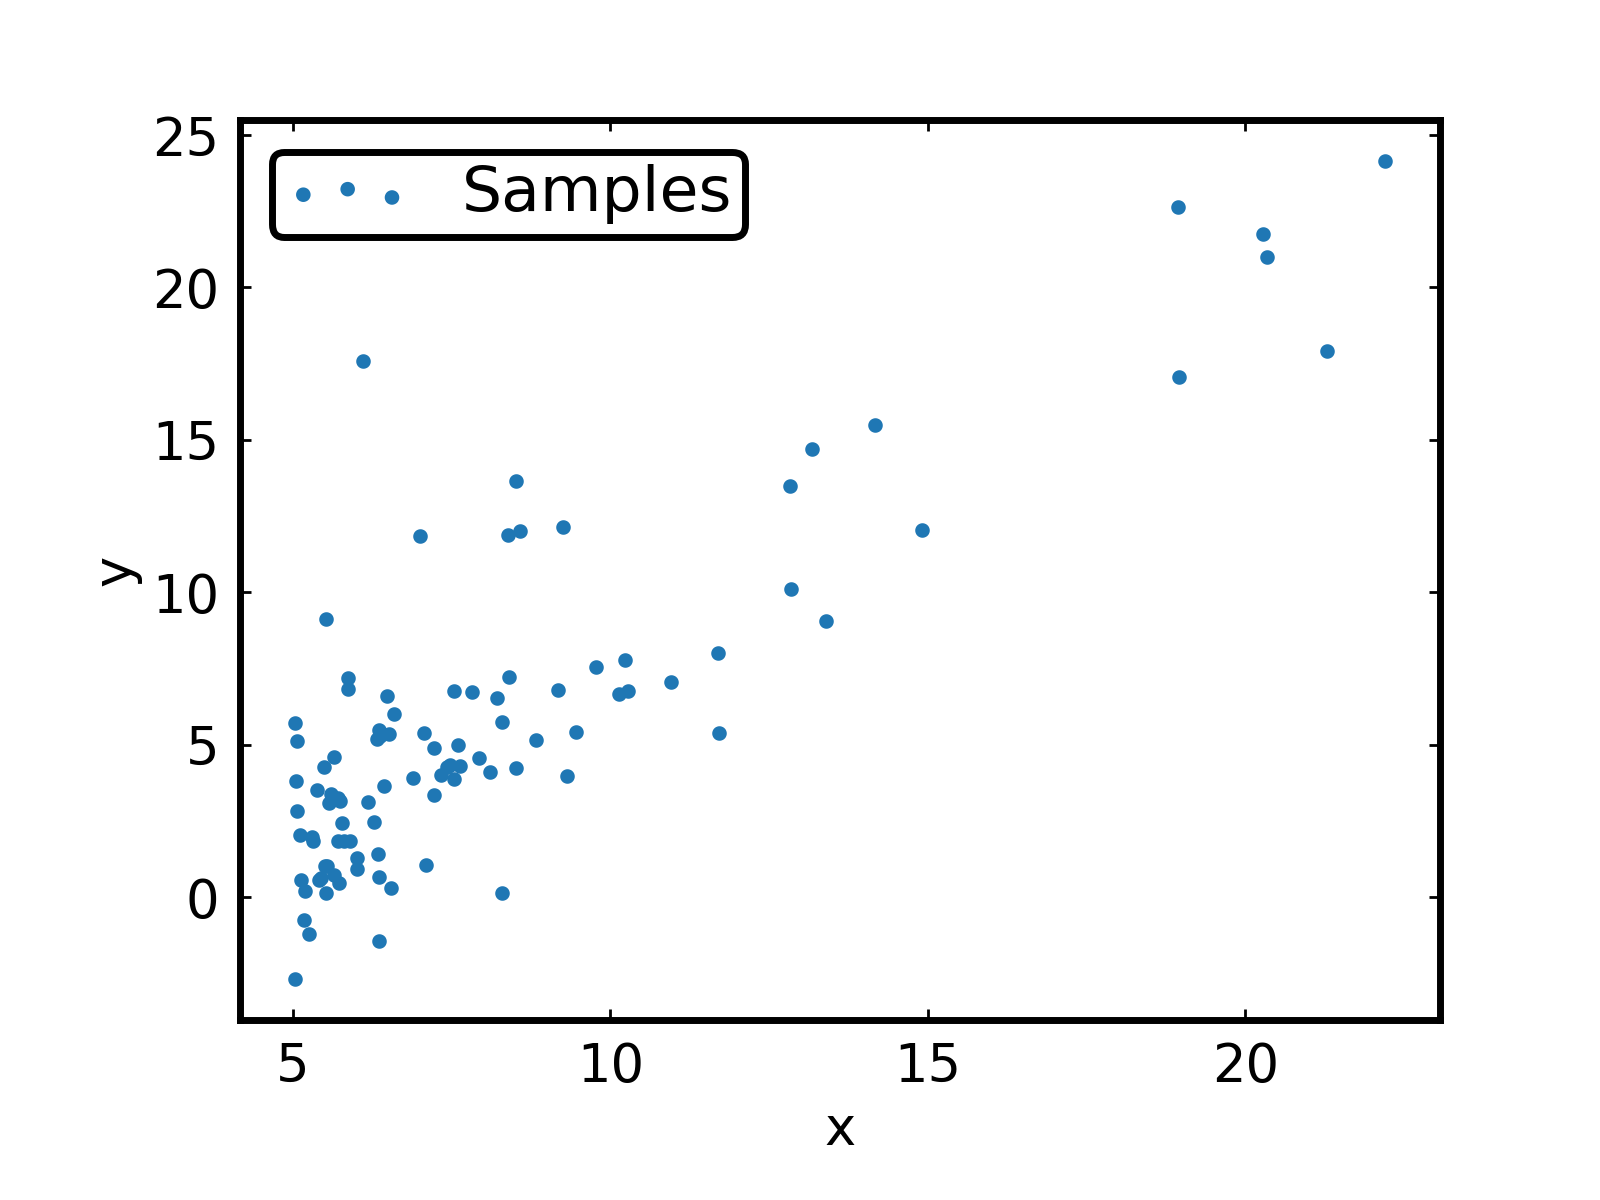
\includegraphics[width=0.85\textwidth]{fig/prob1/data.png}
\centering 
\caption{Data}
\label{fig:data}
\end{figure}

\subsection{Result}

With the parameter as $alpha = 0.001$, $eps = 10^{-8}$, 
$n_{epoch} = 10000$, we can get the regression with final loss as 4.516. The learned parameters are 

\begin{equation}
w = 1.127, b = -3.240
\end{equation}

\begin{figure}[H]
\centering
  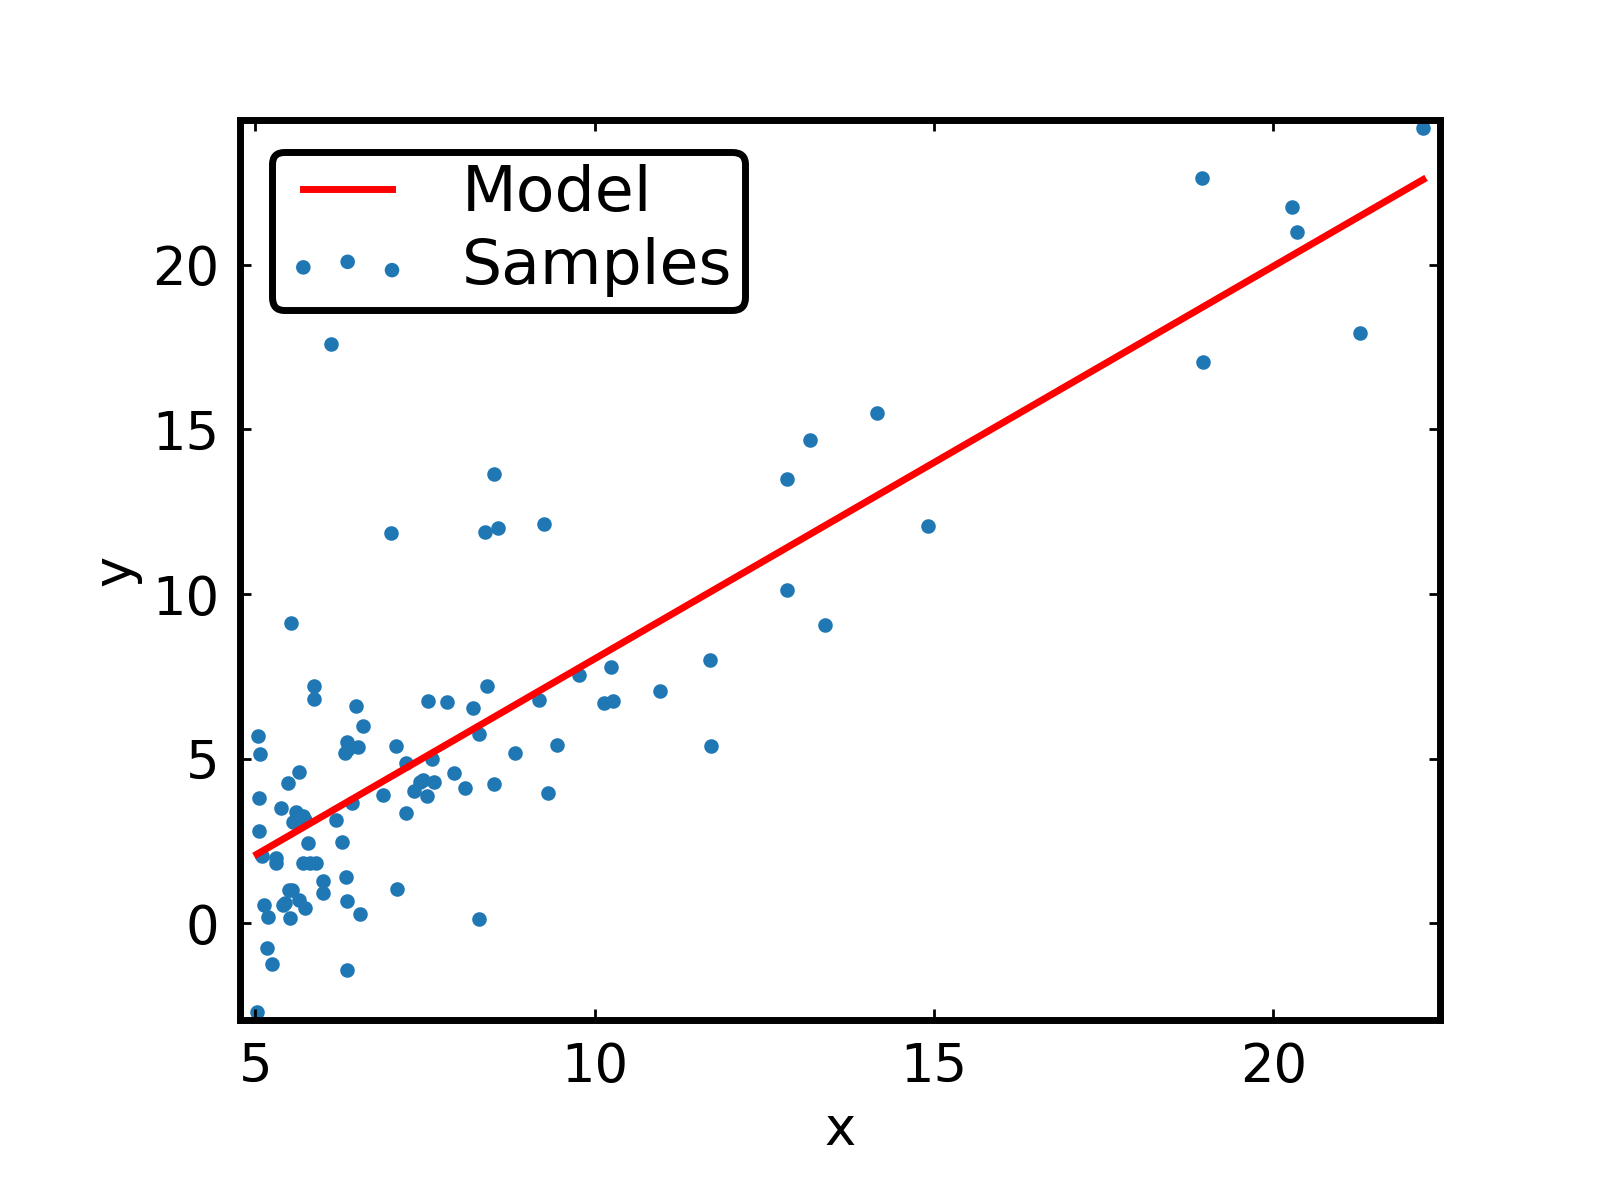
\includegraphics[width=0.85\textwidth]{fig/prob1/fit.png}
\centering 
\caption{Fitting result v.s. data}
\label{fig:fit}
\end{figure}

\begin{figure}[H]
\centering
  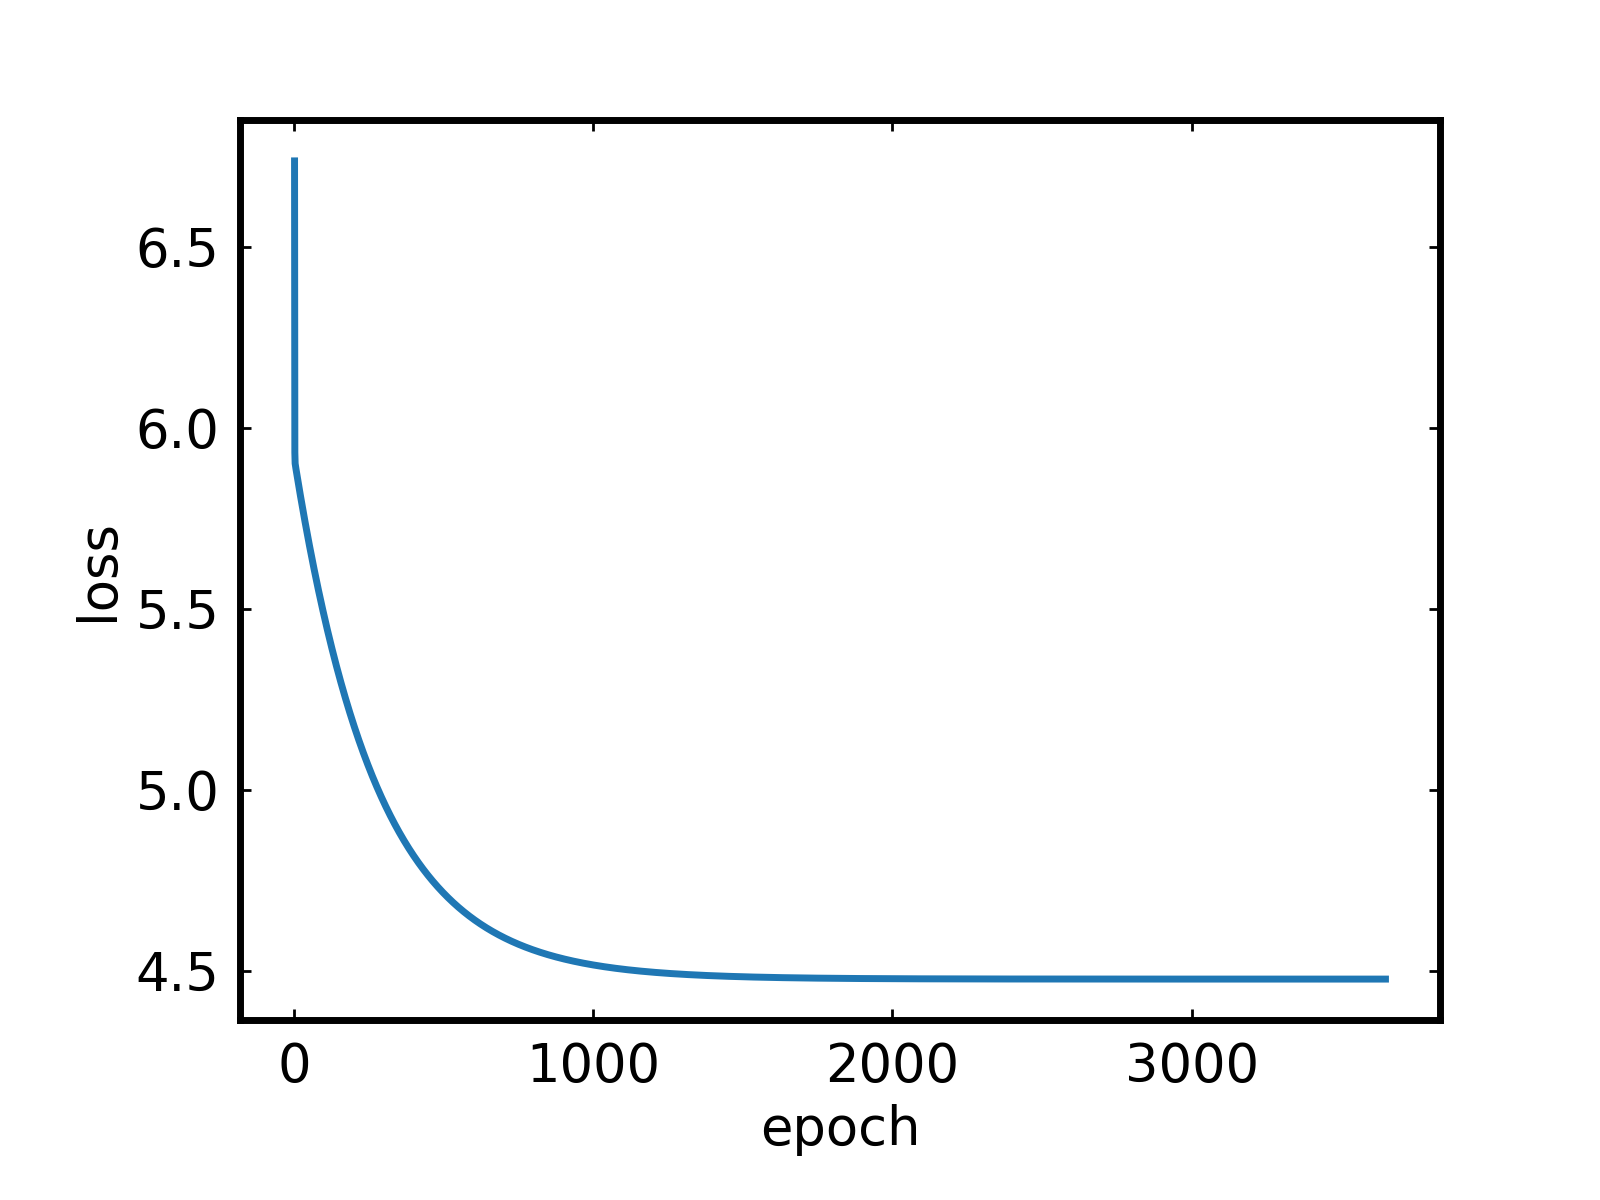
\includegraphics[width=0.85\textwidth]{fig/prob1/loss.png}
\centering 
\caption{Loss v.s. epochs}
\label{fig:loss}
\end{figure}

Here is the process of tuning the parameter alpha. 

\begin{table}[htb]
\centering
\caption{Loss for different learning rate alpha}
\begin{tabular}{|l|l|}
\hline
$\alpha$ & loss \\ \hline
0.0001 & 5.48 \\ \hline
0.001 & 4.51 \\ \hline
0.01 & 4.47 \\ \hline
0.02 & 4.47 \\ \hline
0.05 & nan \\ \hline
0.1 & nan \\ \hline
\hline
\end{tabular}
\label{tab:alpha}
\end{table}

Small learning rate will make the learning process very slow. For example, when $\alpha$ is set to 0.0001, after 10,000 epochs, the loss is still decreasing. Larger learning rate will speed up the learning process, but may lead to unstable results. Usually, it takes several hundreds (\~500) epochs to converge to a reasonable solution.


\section{Problem 2}

\subsection{Fitting Result}

With the parameter as $alpha = 0.001$, $eps = 10^{-8}$, 
$n_{epoch} = 500000$, we can get the regression with the following results.

\begin{figure}[H]
\centering
  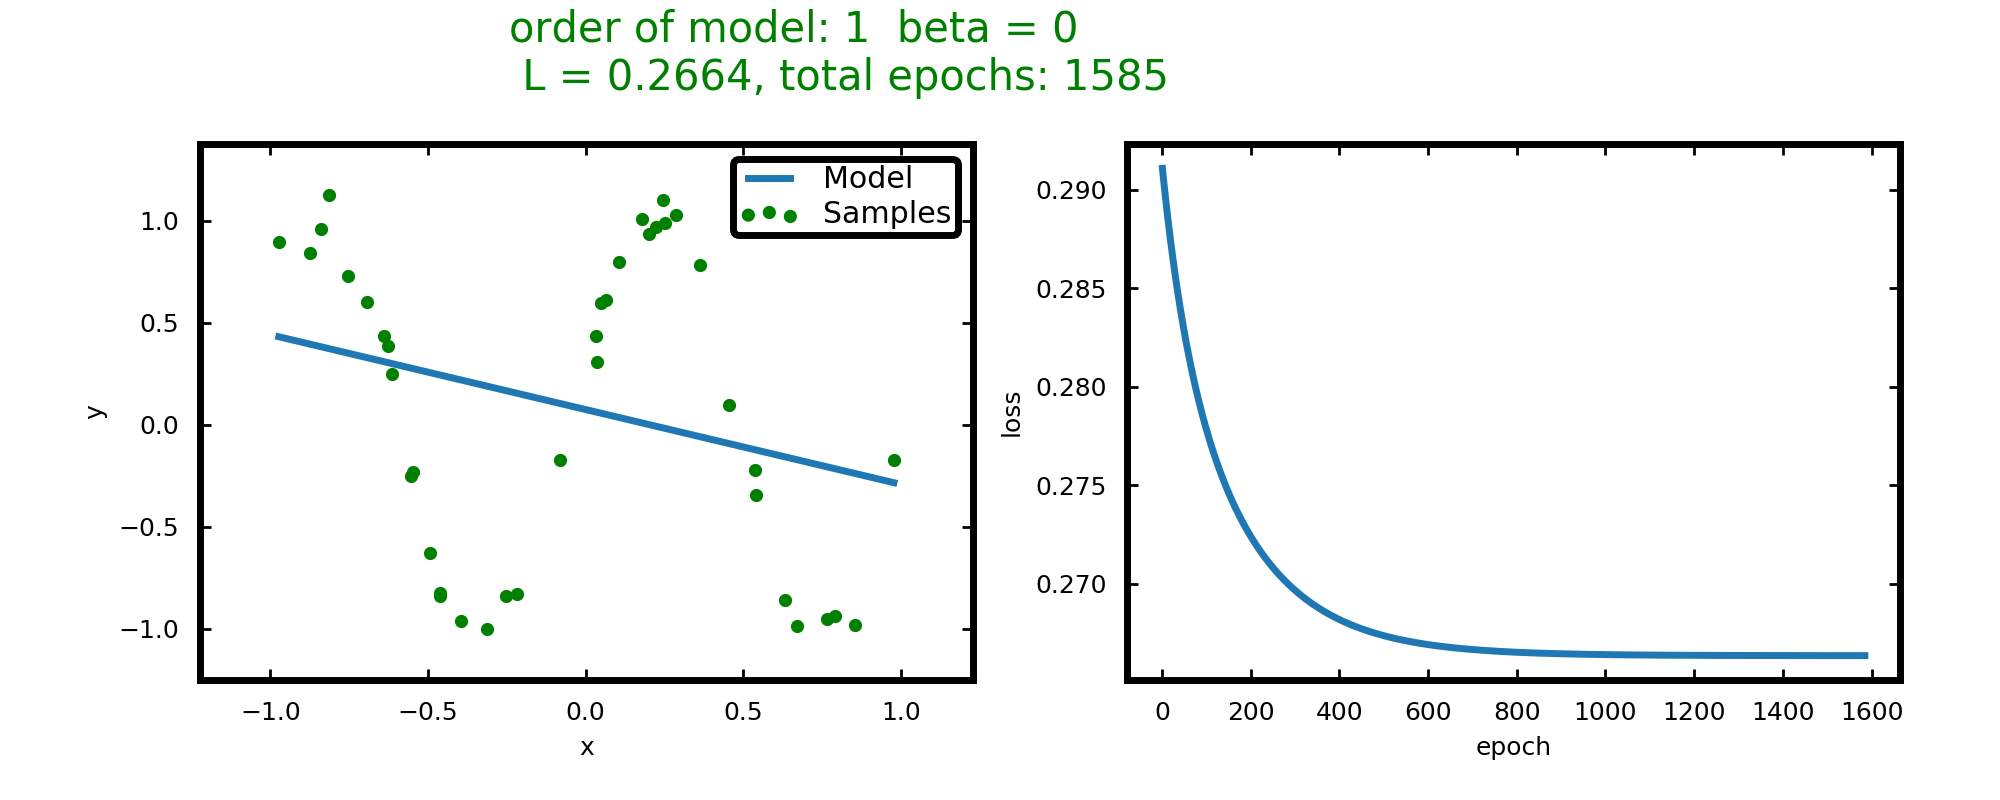
\includegraphics[width=0.85\textwidth]{fig/prob2/degree_1_beta_0_loss.png}
\centering 
\caption{1st order}
\label{fig:1st}
\end{figure}
\begin{figure}[H]
\centering
  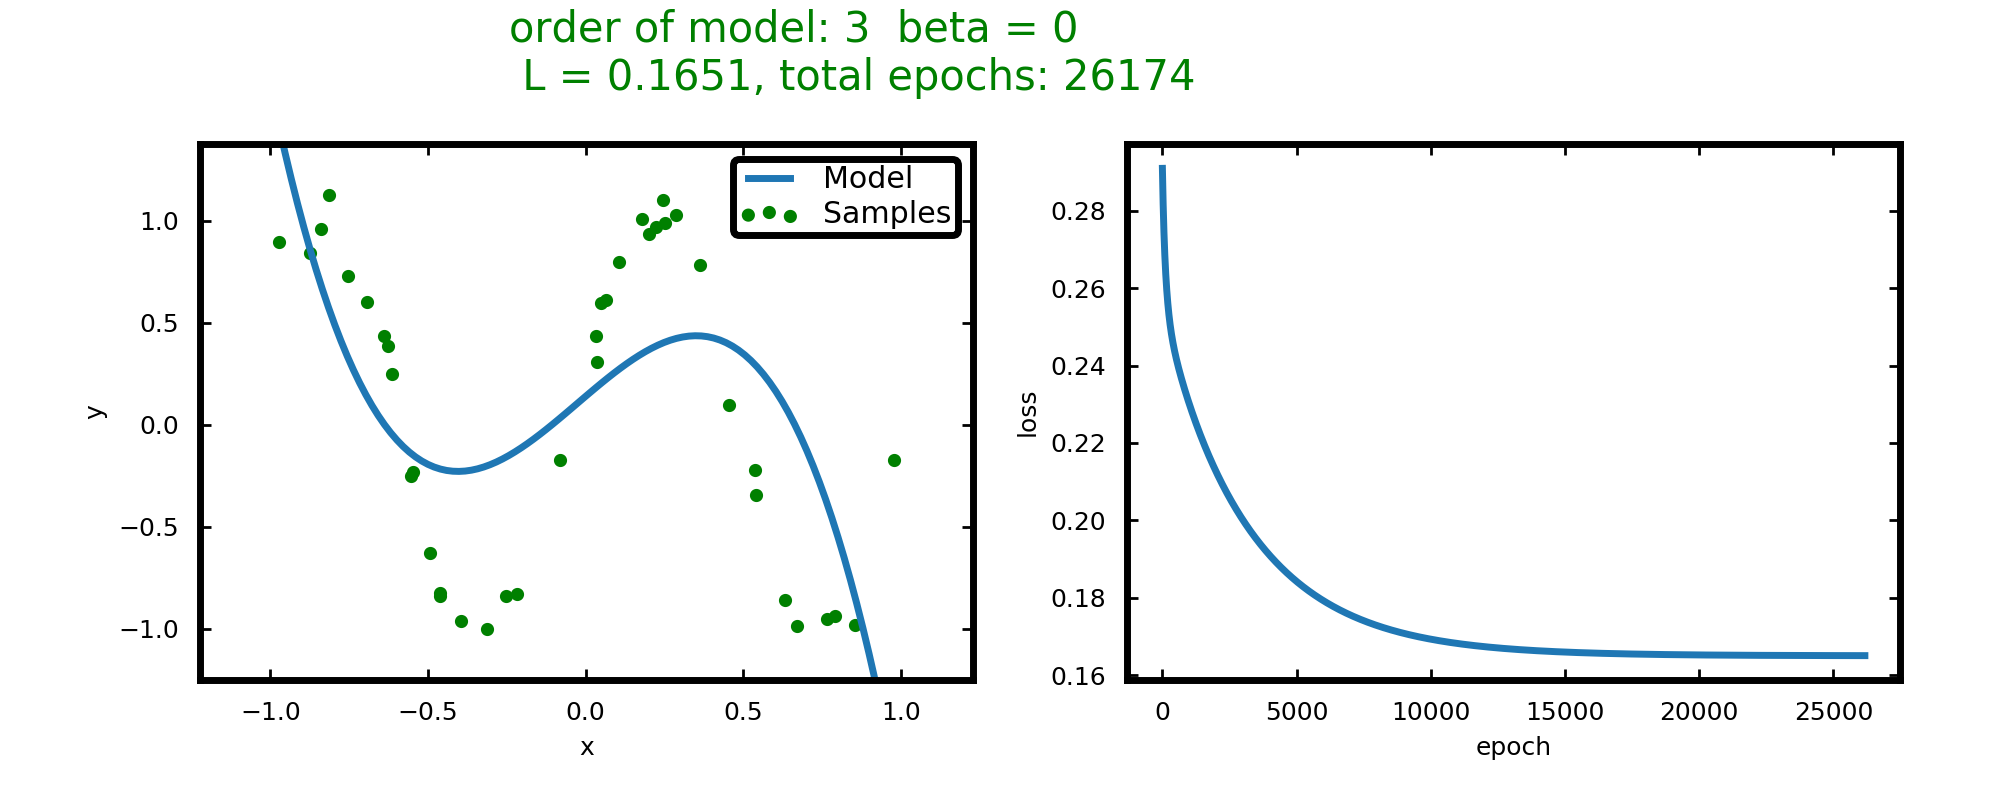
\includegraphics[width=0.85\textwidth]{fig/prob2/degree_3_beta_0_loss.png}
\centering 
\caption{3rd order}
\label{fig:3rd}
\end{figure}
\begin{figure}[H]
\centering
  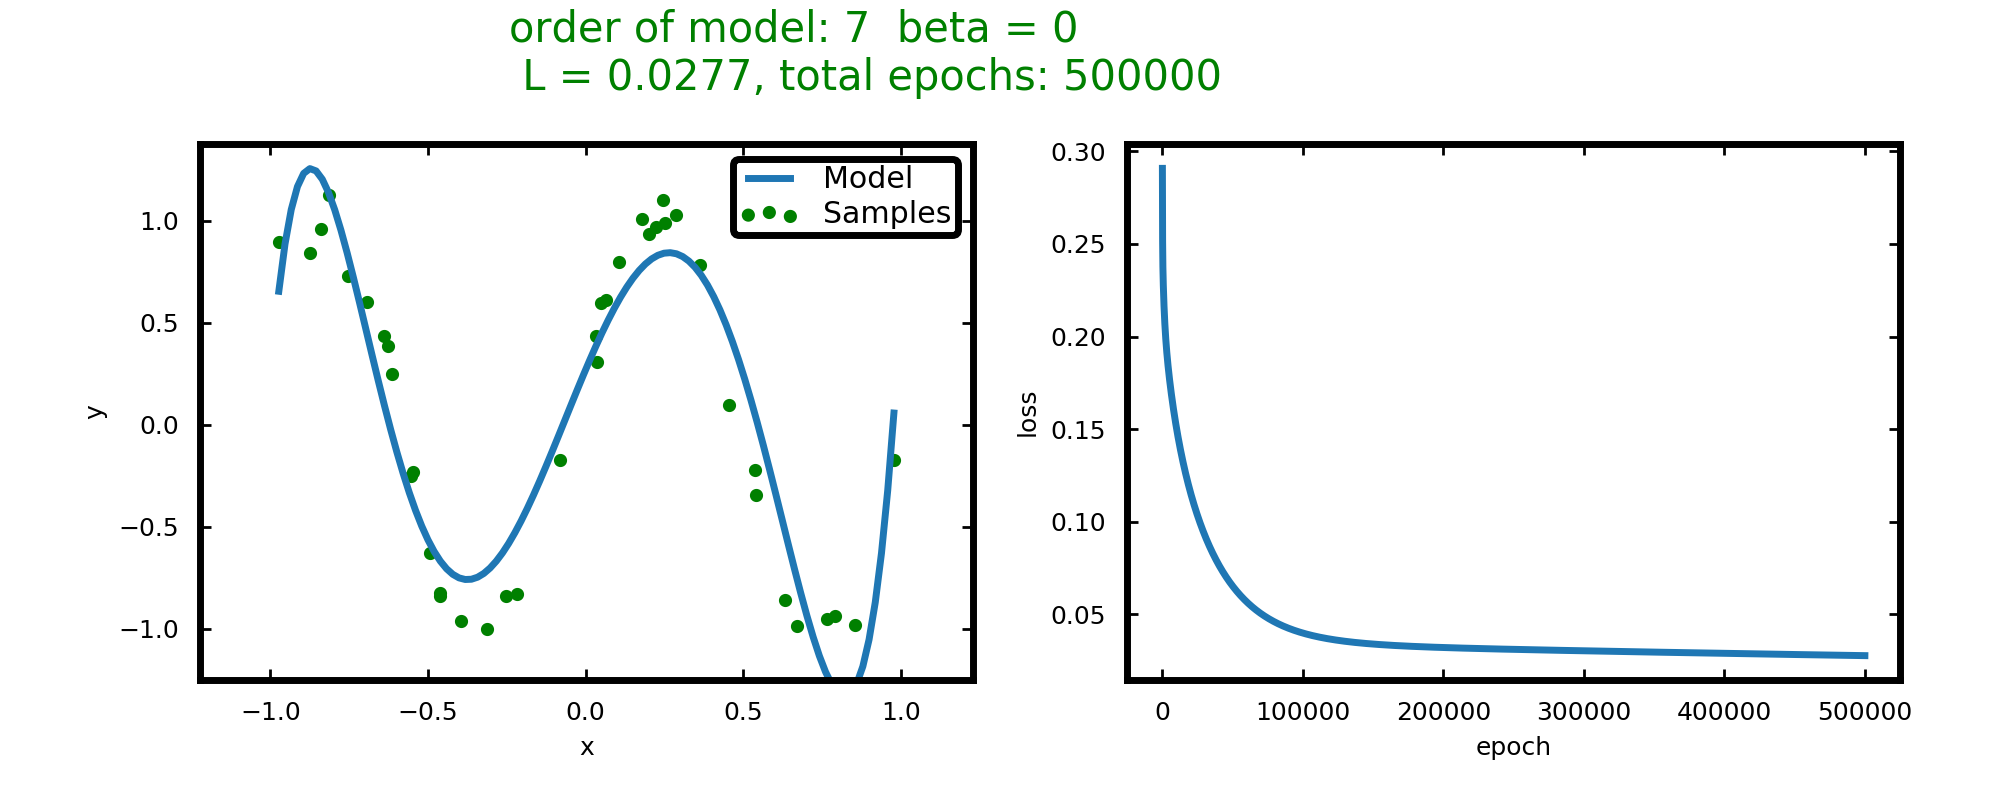
\includegraphics[width=0.85\textwidth]{fig/prob2/degree_7_beta_0_loss.png}
\centering 
\caption{7th order}
\label{fig:7th}
\end{figure}
\begin{figure}[H]
\centering
  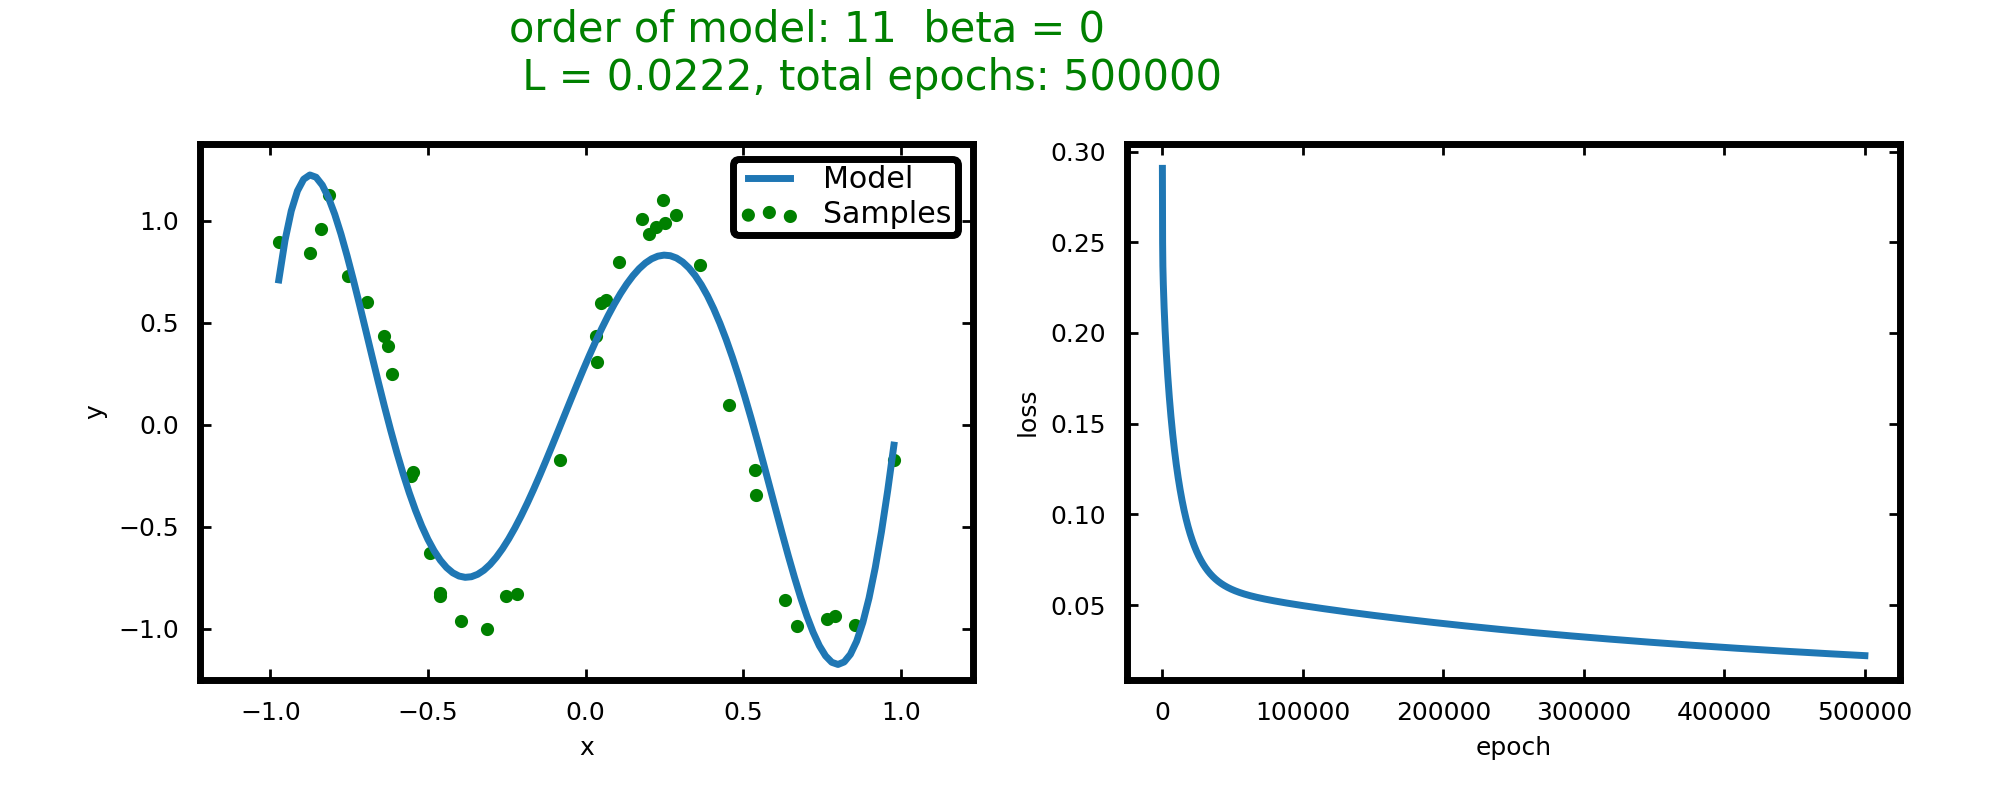
\includegraphics[width=0.85\textwidth]{fig/prob2/degree_11_beta_0_loss.png}
\centering 
\caption{11th order}
\label{fig:11th}
\end{figure}
\begin{figure}[H]
\centering
  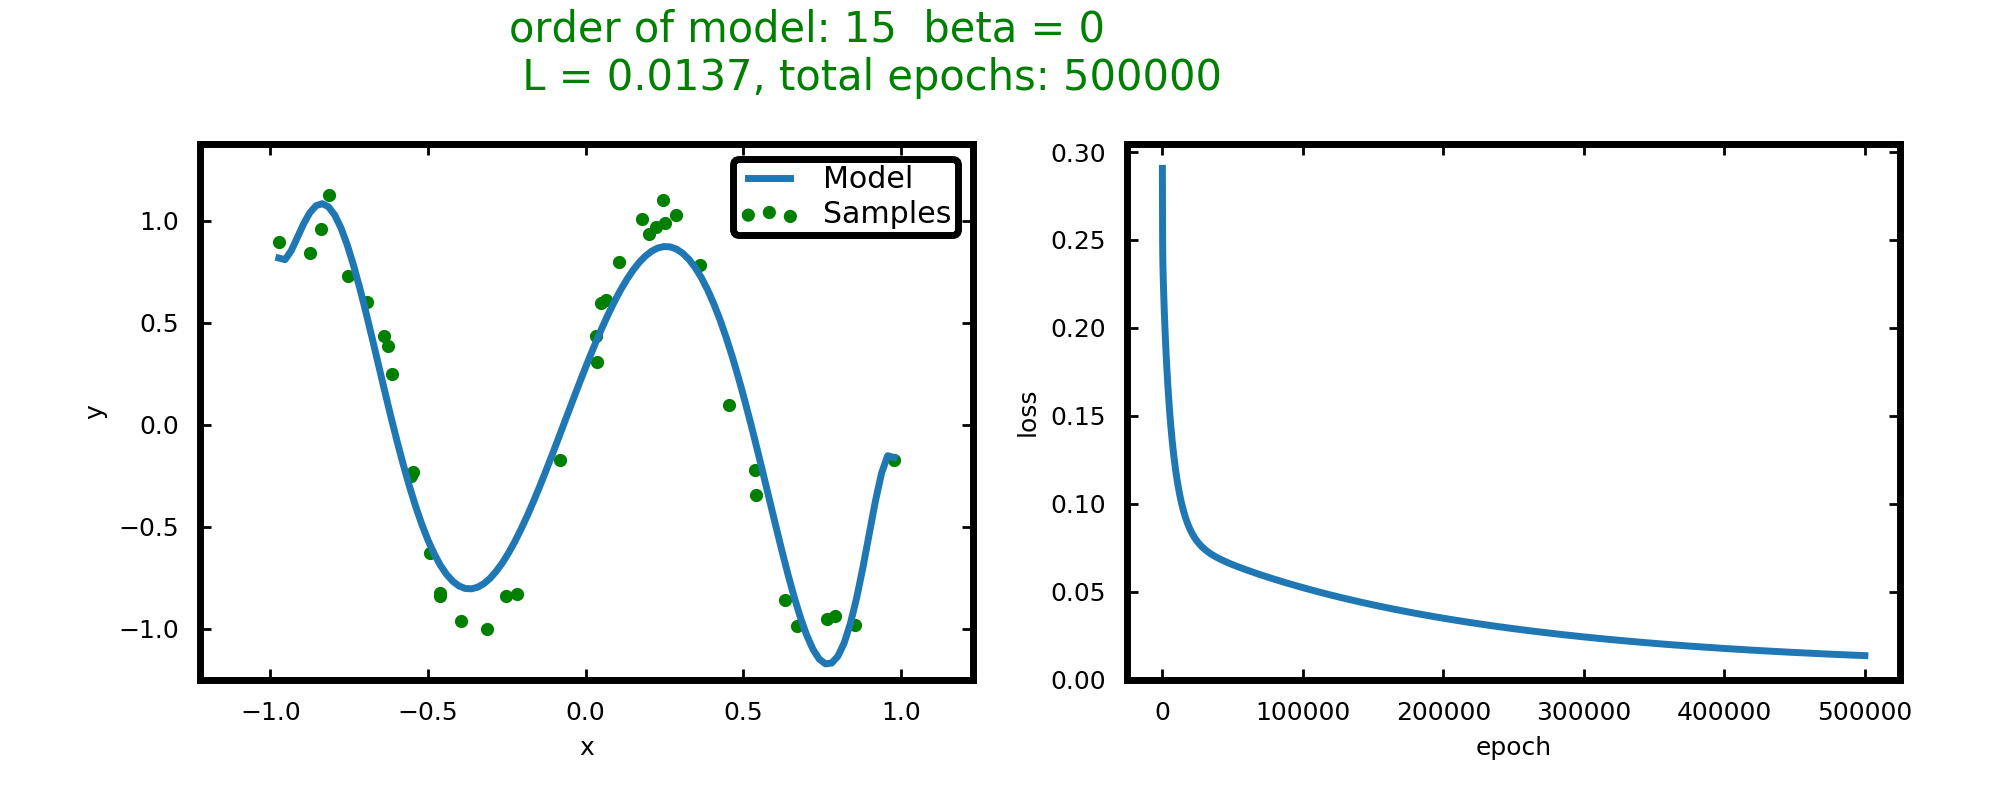
\includegraphics[width=0.85\textwidth]{fig/prob2/degree_15_beta_0_loss.png}
\centering 
\caption{15th order}
\label{fig:15th}
\end{figure}


\begin{itemize}
\item With respect to the feature mapping, what is a potential problem that the scheme we have designed above might create?
What is one solution to fixing any potential problems created by using this scheme (and what other problems might that solution induce)?

The created features ($x$, $x^2$, $x^3$, ...) are highly correlated. In this way, the coefficient of each feature will highly depend on what features are included in the model. (i.e., including $x^2$ will have strong influence on the coefficient of $x$). This is not the correct relationship between $x$ and $y$ that we want to model.

One possible solution is to just feed one $x$ input into the computation graph, and make the $x$, $x^2$, $x^3$ as a hidden layer. Then, when computing the gradient, the change in $x$ will cause the change in all the hidden layers.

\item What do you observe as the capacity of the model is increased? Why does this happen? 

As the capacity of the model increase, the model is able to fit the data better (the loss is decreasing). This is due to the reason that higher order polynomial can fit more details than lower order polynomial. If we push the order to infinity, this will become taylor series, which is able to fit any function form.

\end{itemize}

\subsection{Tuning the regularization}


\begin{figure}[H]
\centering
  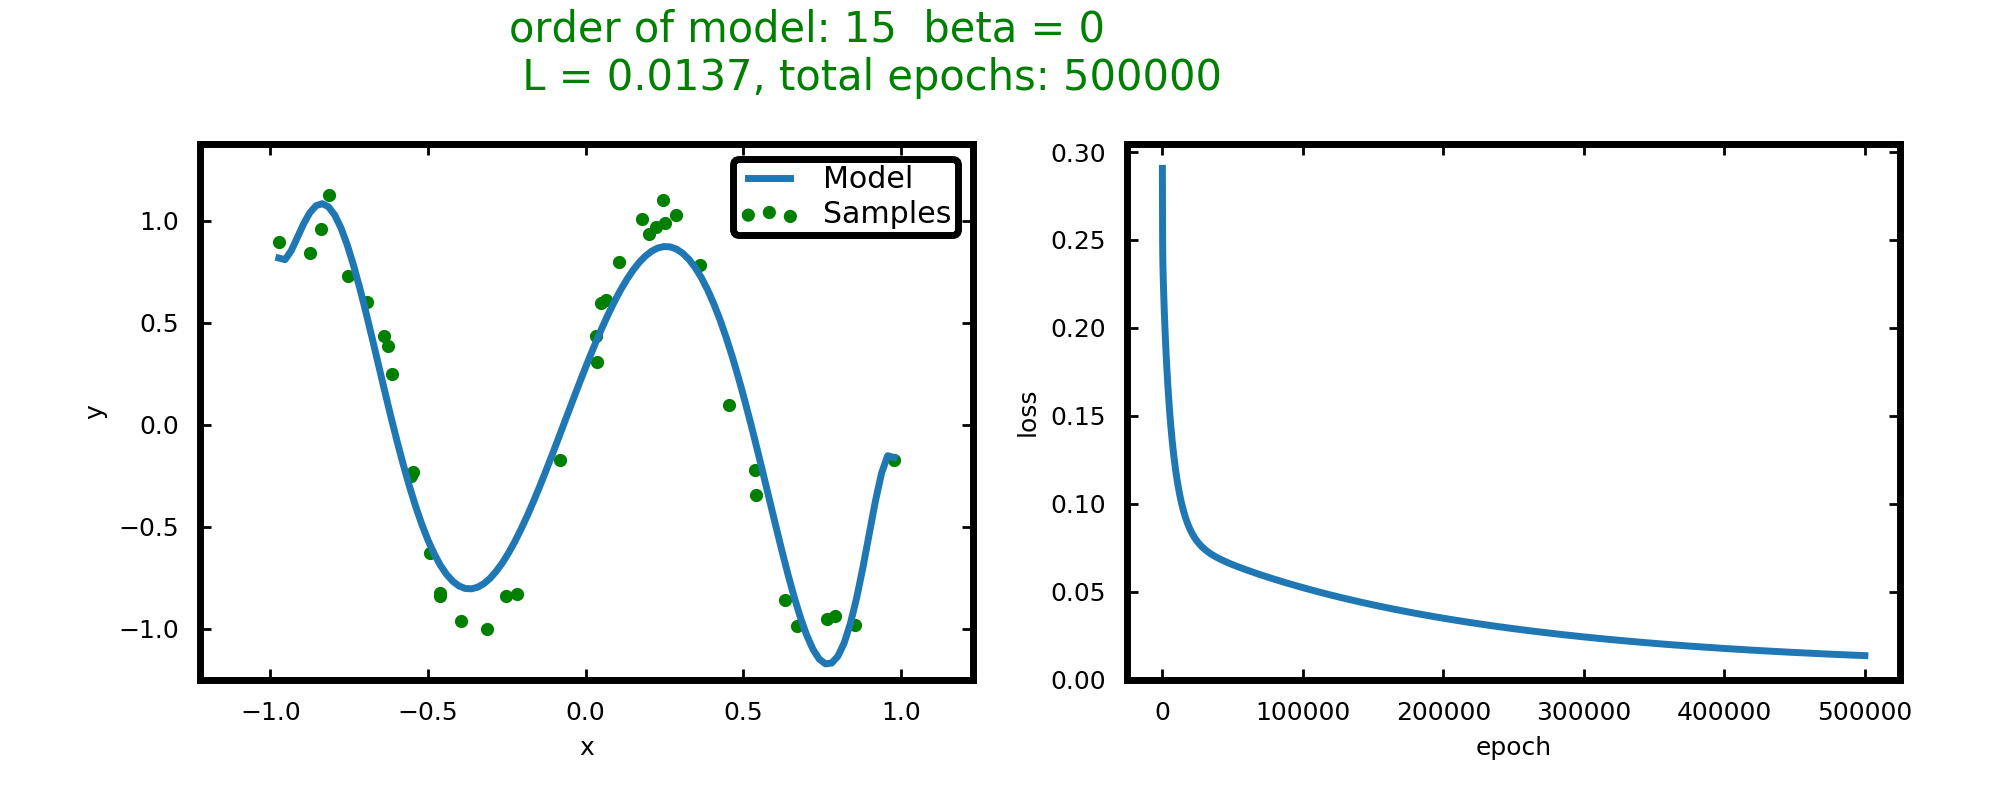
\includegraphics[width=0.85\textwidth]{fig/prob2/degree_15_beta_0_loss.png}
\centering 
\caption{\protect 15th order, $\beta = 0$}
\label{fig:15th}
\end{figure}
\begin{figure}[H]
\centering
  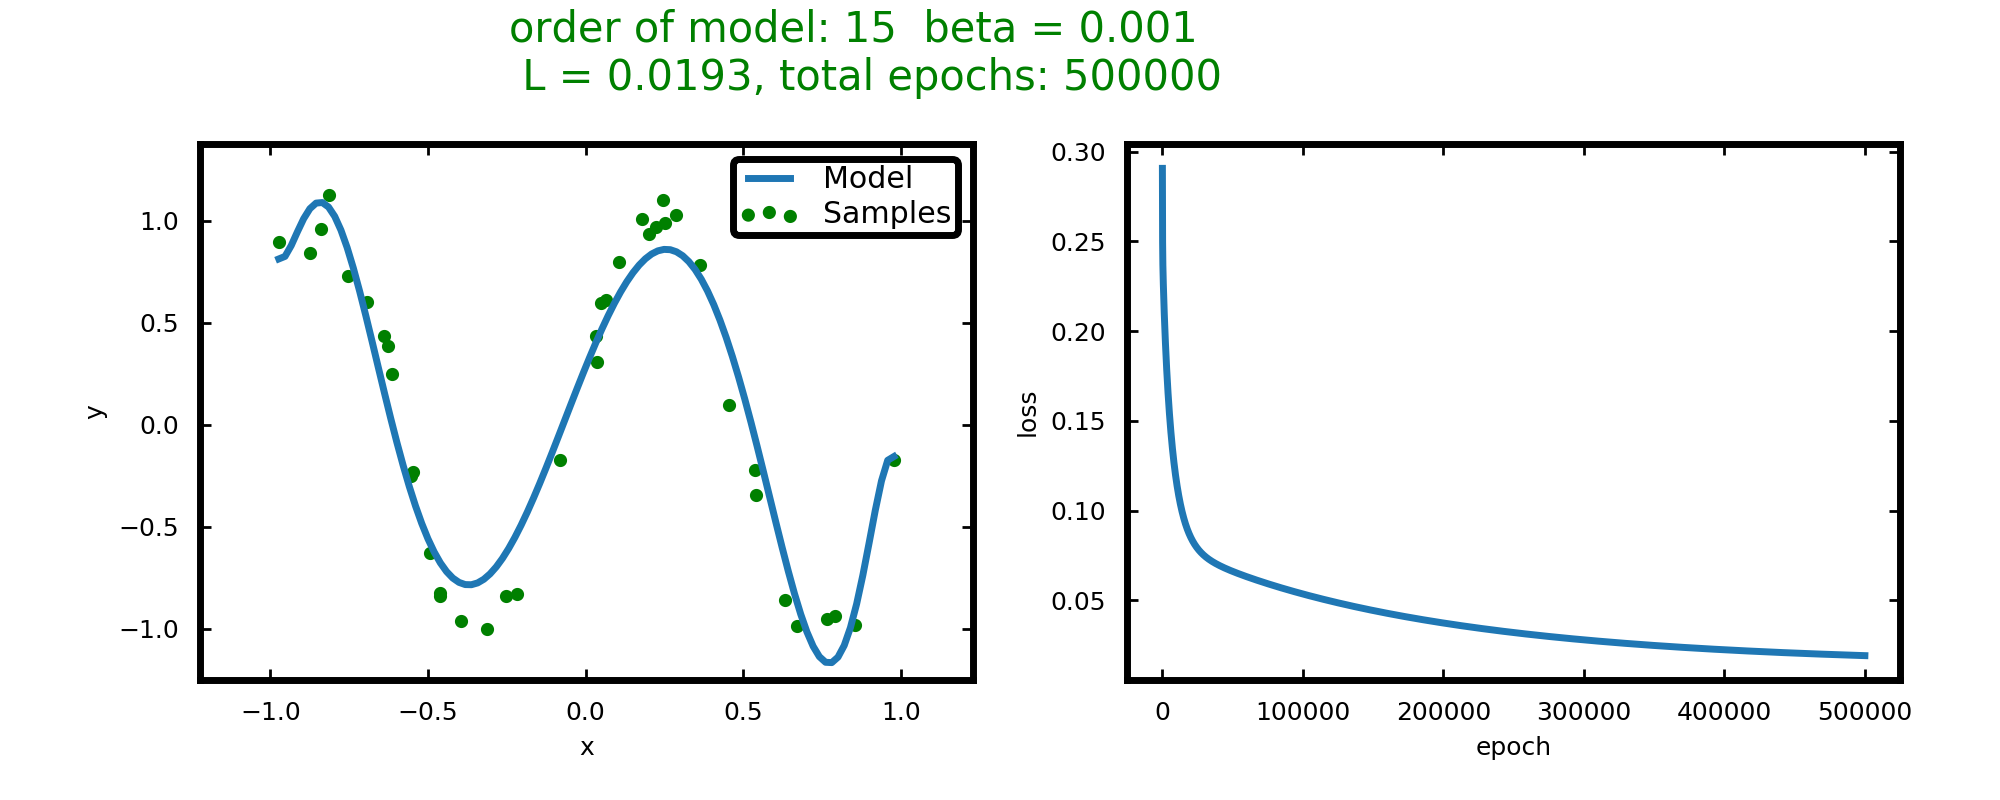
\includegraphics[width=0.85\textwidth]{fig/prob2/degree_15_beta_0_001_loss.png}
\centering 
\caption{\protect 15th order, $\beta = 0.001$}
\label{fig:15th}
\end{figure}
\begin{figure}[H]
\centering
  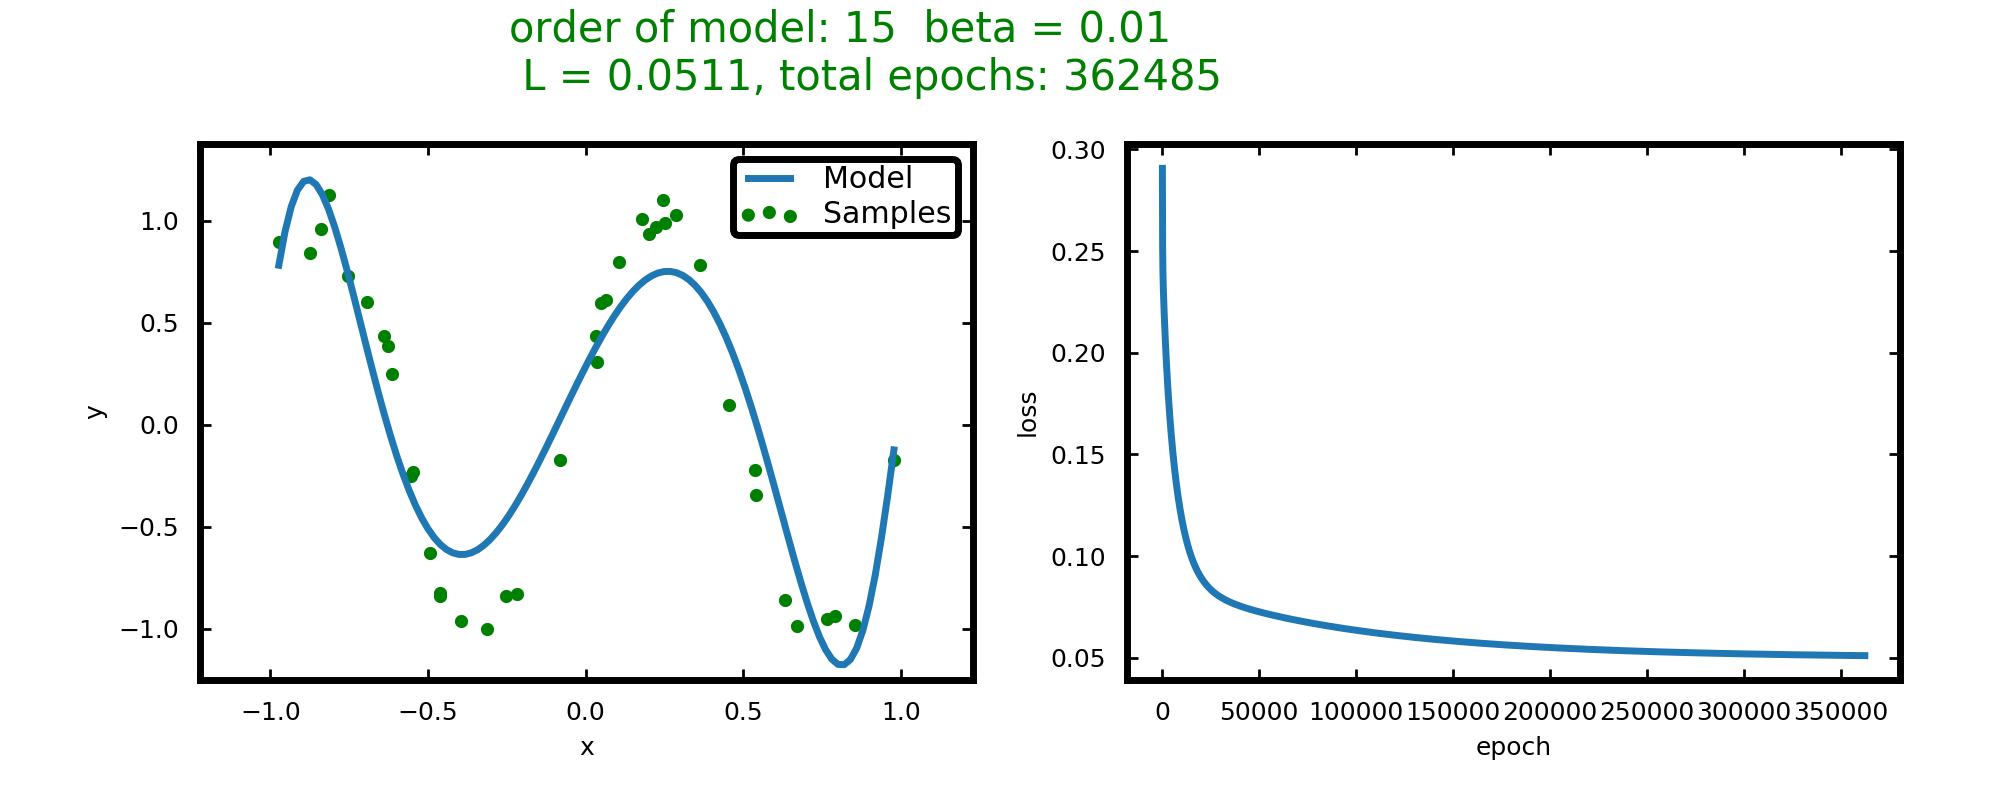
\includegraphics[width=0.85\textwidth]{fig/prob2/degree_15_beta_0_01_loss.png}
\centering 
\caption{\protect 15th order, $\beta = 0.01$}
\label{fig:15th}
\end{figure}
\begin{figure}[H]
\centering
  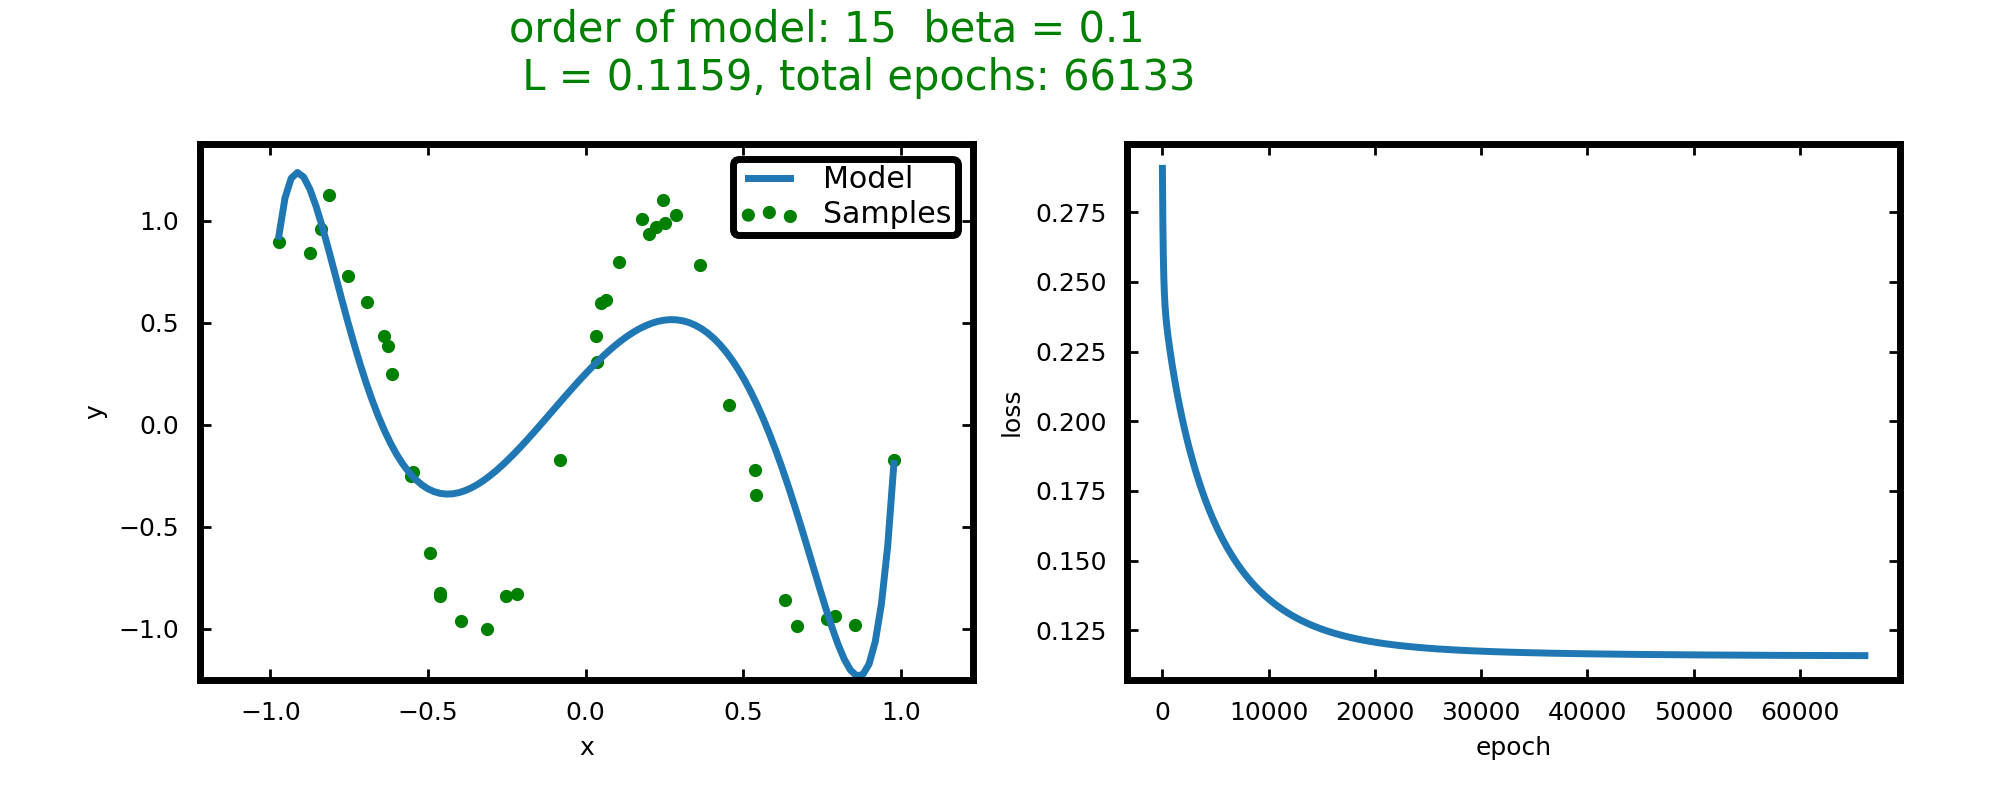
\includegraphics[width=0.85\textwidth]{fig/prob2/degree_15_beta_0_1_loss.png}
\centering 
\caption{\protect 15th order, $\beta = 0.1$}
\label{fig:15th}
\end{figure}
\begin{figure}[H]
\centering
  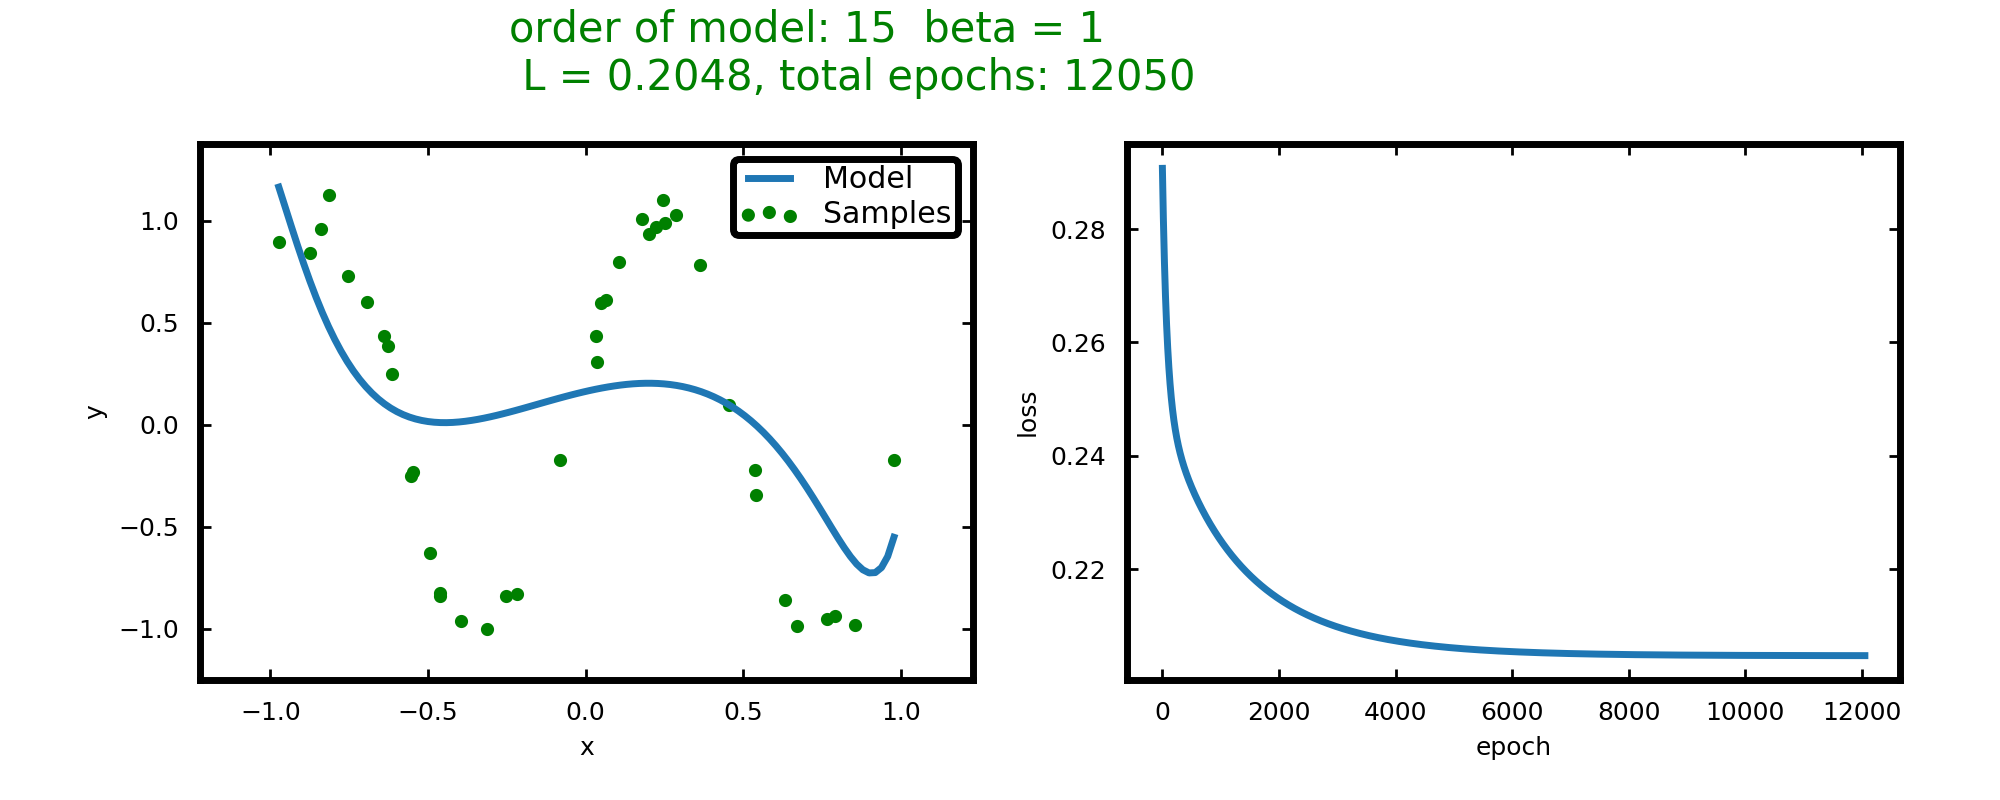
\includegraphics[width=0.85\textwidth]{fig/prob2/degree_15_beta_1_loss.png}
\centering 
\caption{\protect 15th order, $\beta = 1$}
\label{fig:15th}
\end{figure}

\begin{itemize}
\item What do you observe as you
increase the value of $\beta$? How does this interact with the general model fitting process (such as the step
size $\alpha$ and number of epochs needed to reach convergence)?

As $\beta$ increase, the model tends to be more general (have less detailed information). The general model fitting process becomes faster and will converge with fewer epochs. 

\item What might be a problem with a convergence check that compares the current cost with the previous cost (i.e., looks at the deltas between costs at time t and t − 1), especially for a more complicated model? How can we fix this?

\textbf{I already added this convergence check in the code.} If the function is not convex everywhere, then this convergence check might lead to a local optimum if the step size is not very big. Because the optimizer might get trapped in the local optimum for several epochs. We can wait for several epochs. Within these several epochs, if the loss decrease is always smaller than a threshold value, we stop the optimiation.
  
\end{itemize}








\section{Problem 3}

\subsection{Fitting result without regularization}

I tuned the $\alpha$ from [0.001, 0.01, 0.1] and $n_{epoch}$ from [100000, 500000, 1000000]. But actually, with the help of early stopping criterion, we only needs the largest number of epochs. So I only show the result for $n_{epoch} = 1000000$, with varying $\alpha$. Different learning rates do not make the results that different. The lowest error rate is 16.1\%.

\begin{figure}[H]
\centering
  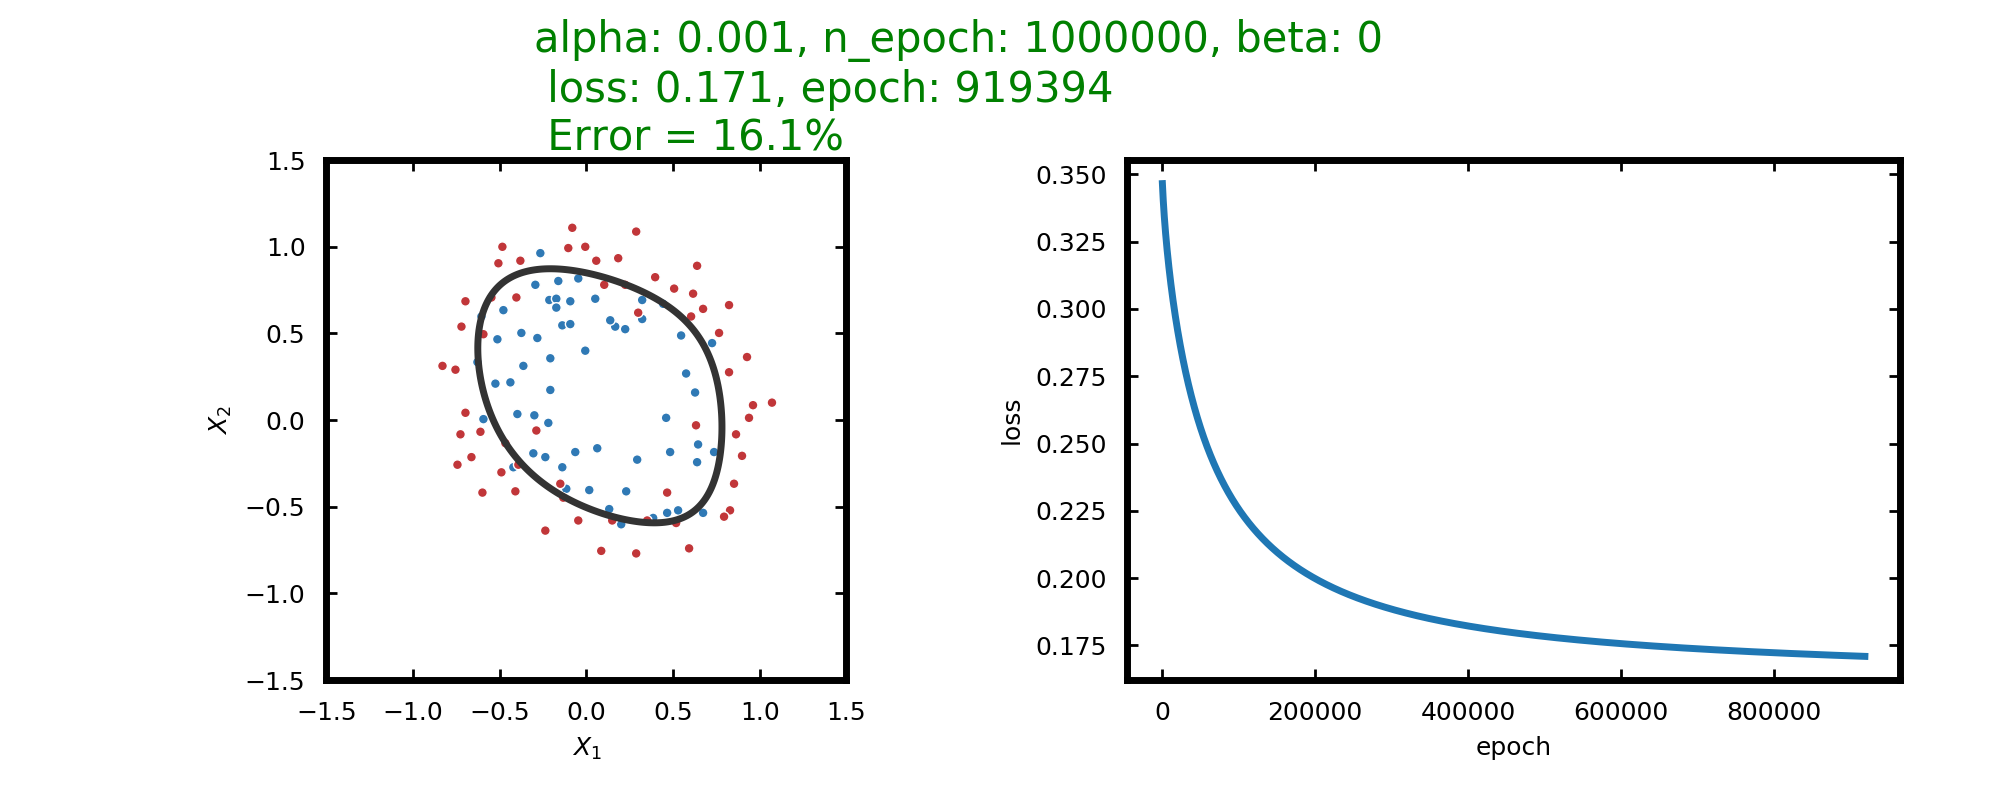
\includegraphics[width=0.85\textwidth]{fig/prob3/alpha_0_001_n_epoch1000000_beta_0.png}
\centering 
\caption{\protect $\alpha = 0.001$, $epoch = 1000000$}
\label{fig:15th}
\end{figure}

\begin{figure}[H]
\centering
  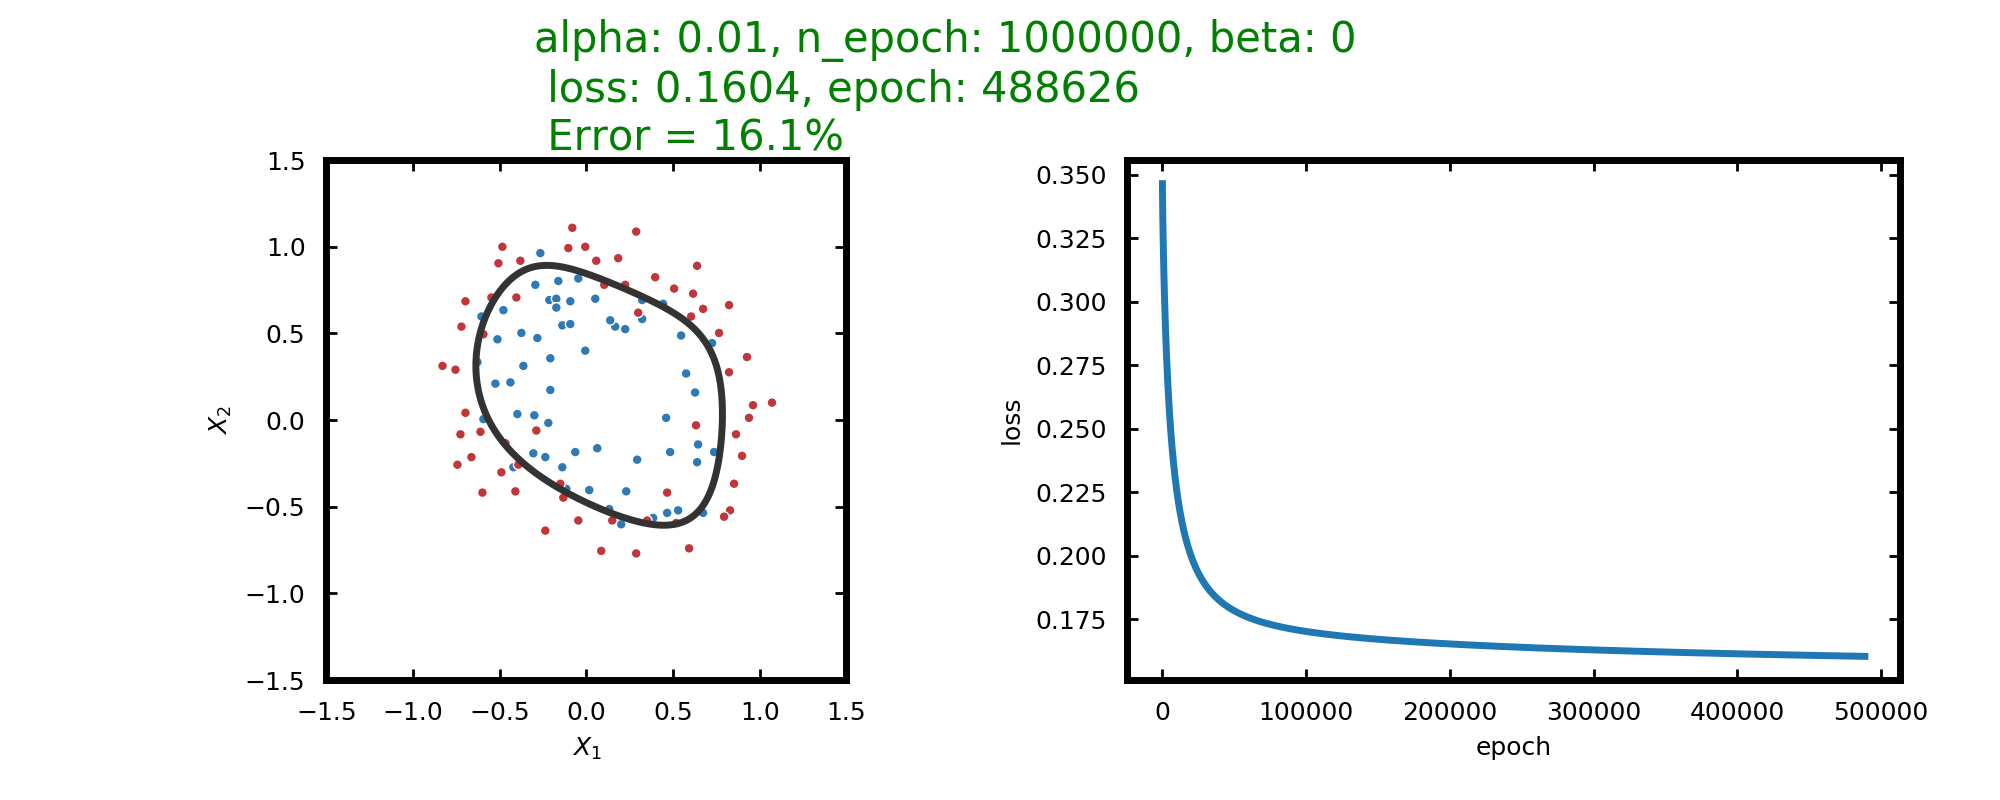
\includegraphics[width=0.85\textwidth]{fig/prob3/alpha_0_01_n_epoch1000000_beta_0.png}
\centering 
\caption{\protect $\alpha = 0.01$, $epoch = 1000000$}
\label{fig:15th}
\end{figure}

\begin{figure}[H]
\centering
  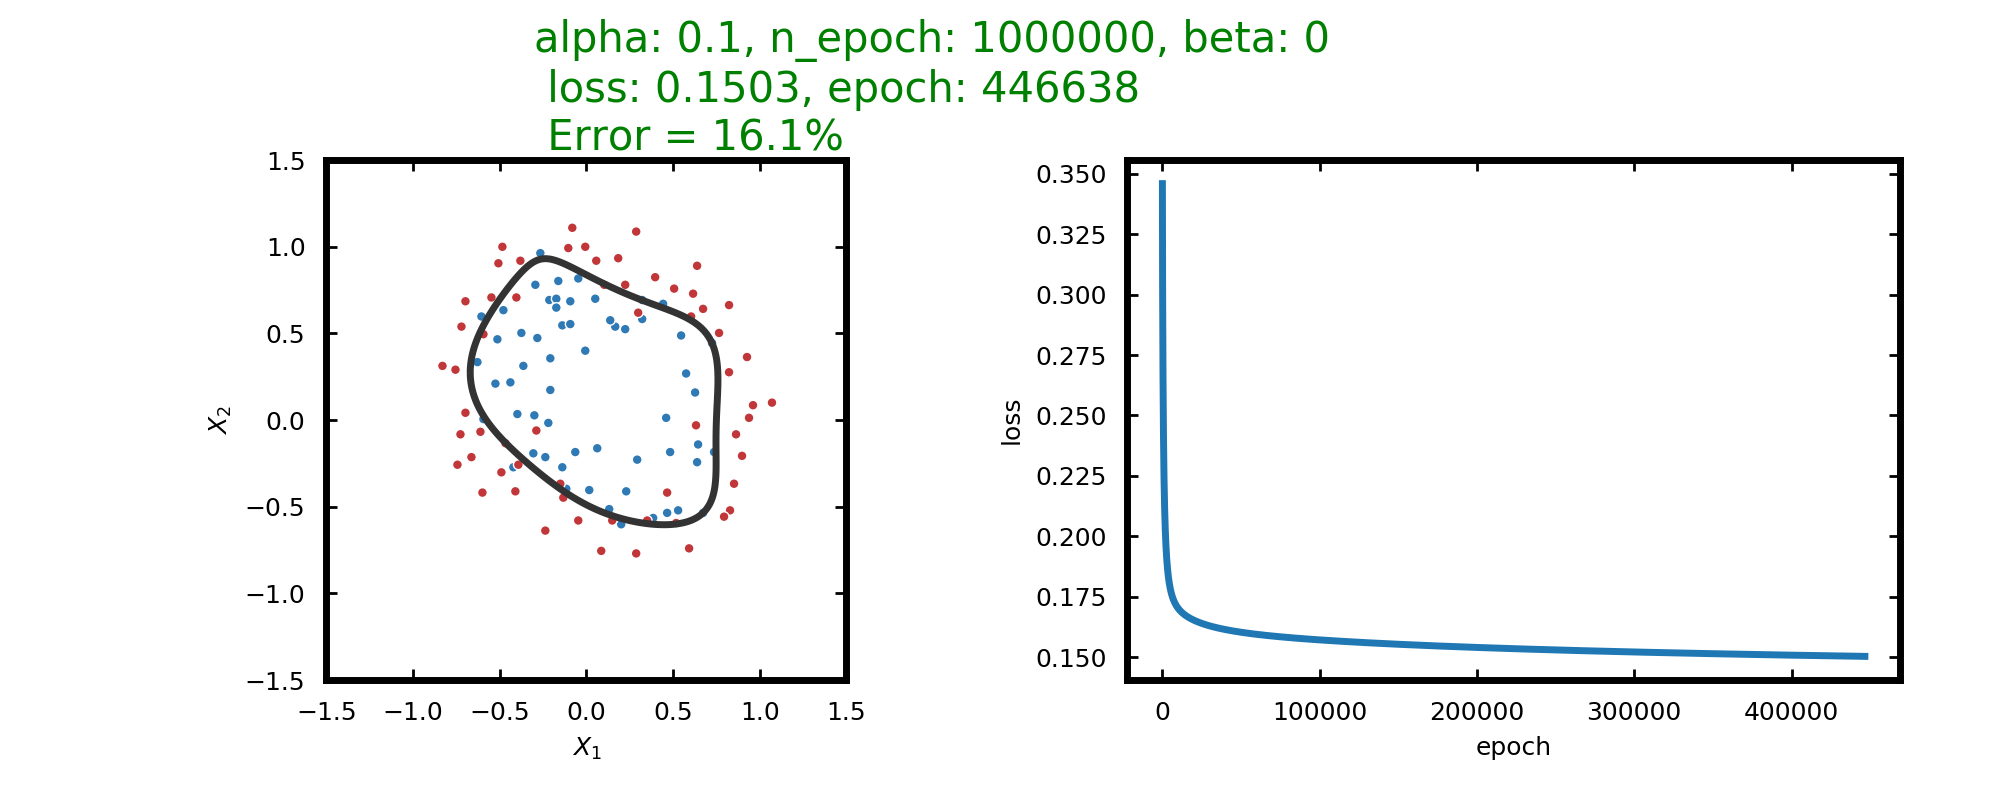
\includegraphics[width=0.85\textwidth]{fig/prob3/alpha_0_1_n_epoch1000000_beta_0.png}
\centering 
\caption{\protect $\alpha = 0.1$, $epoch = 1000000$}
\label{fig:15th}
\end{figure}

\subsection{Tuning the regularization}

I further tune the $\beta$ to change the regularization strength. With some proper strength of regularization (when $\beta \leq 0.1 $), the classification accuracy stays the same. When larger regularization is added, the accuracy starts to decrease. With increasing regularization, the decision boundary tends to be more smooth. 

Regularizing model will make the model more general and prevent it from overfitting.

The results is as below.

\begin{table}[htb]
\centering
\caption{Loss for different regularization}
\begin{tabular}{|l|l|}
\hline
$\beta$ & error rate \\ \hline
0. & 16.1\% \\ \hline
0.1 & 16.1\% \\ \hline
1 &  17.8\% \\ \hline
10 & 27.97\% \\ \hline
100 & 49.15\% \\ \hline
\hline
\end{tabular}
\label{tab:alpha}
\end{table}

\begin{figure}[H]
\centering
  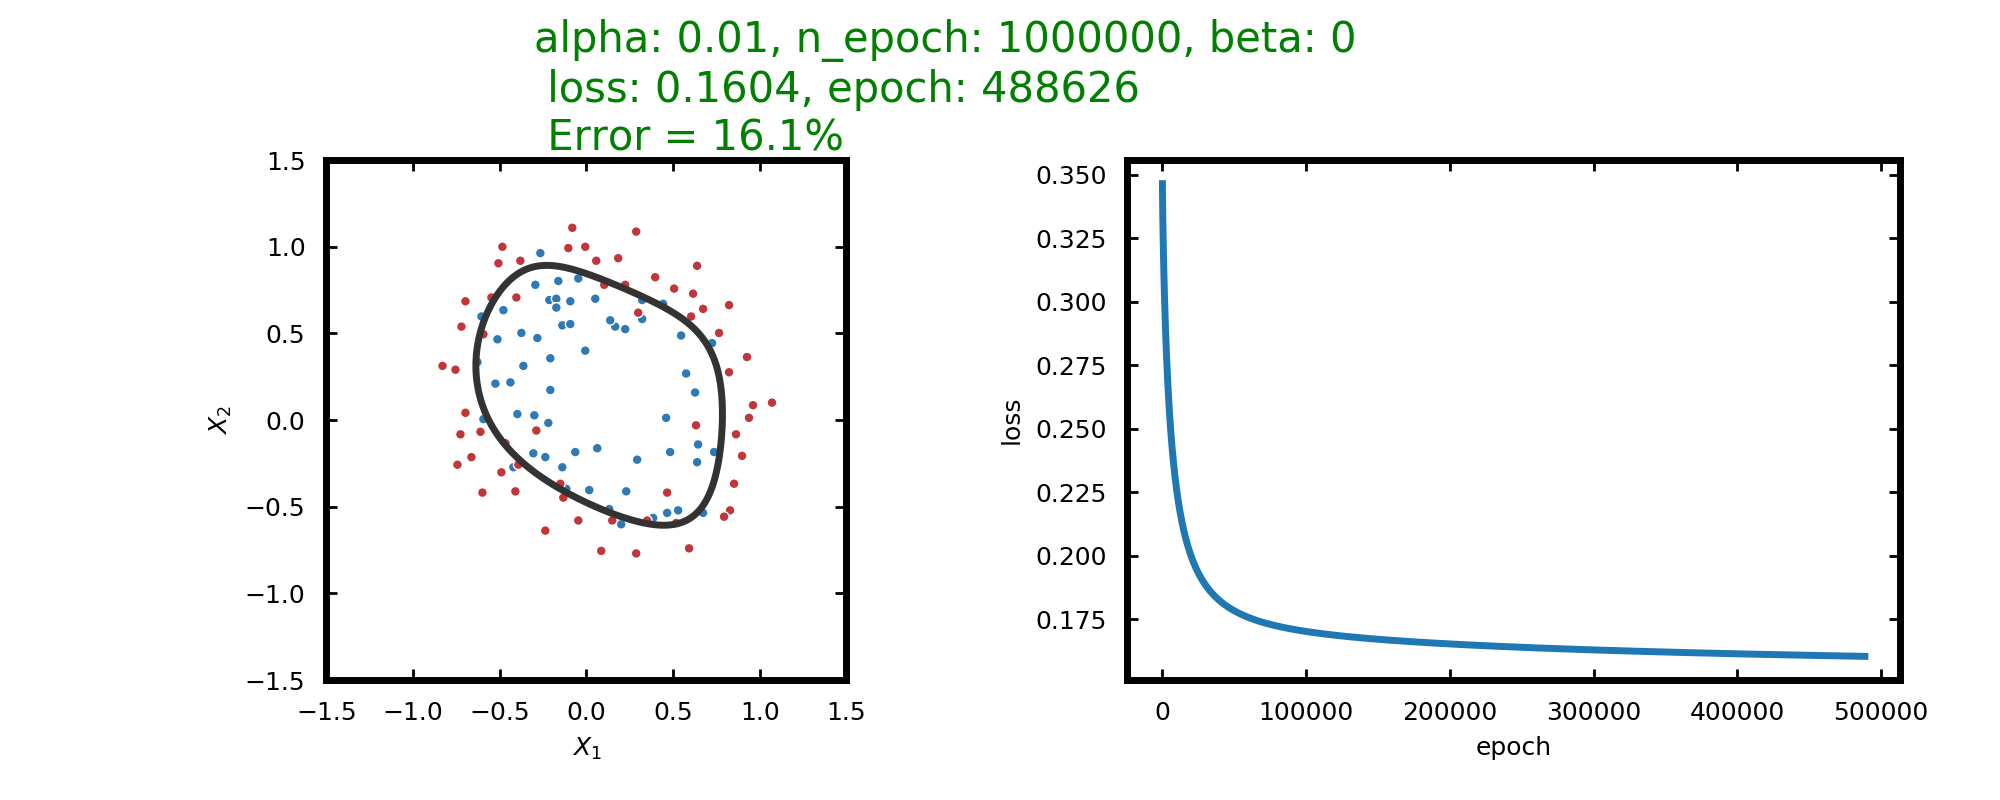
\includegraphics[width=0.85\textwidth]{fig/prob3/alpha_0_01_n_epoch1000000_beta_0.png}
\centering 
\caption{\protect No regularization}
\label{fig:15th}
\end{figure}

\begin{figure}[H]
\centering
  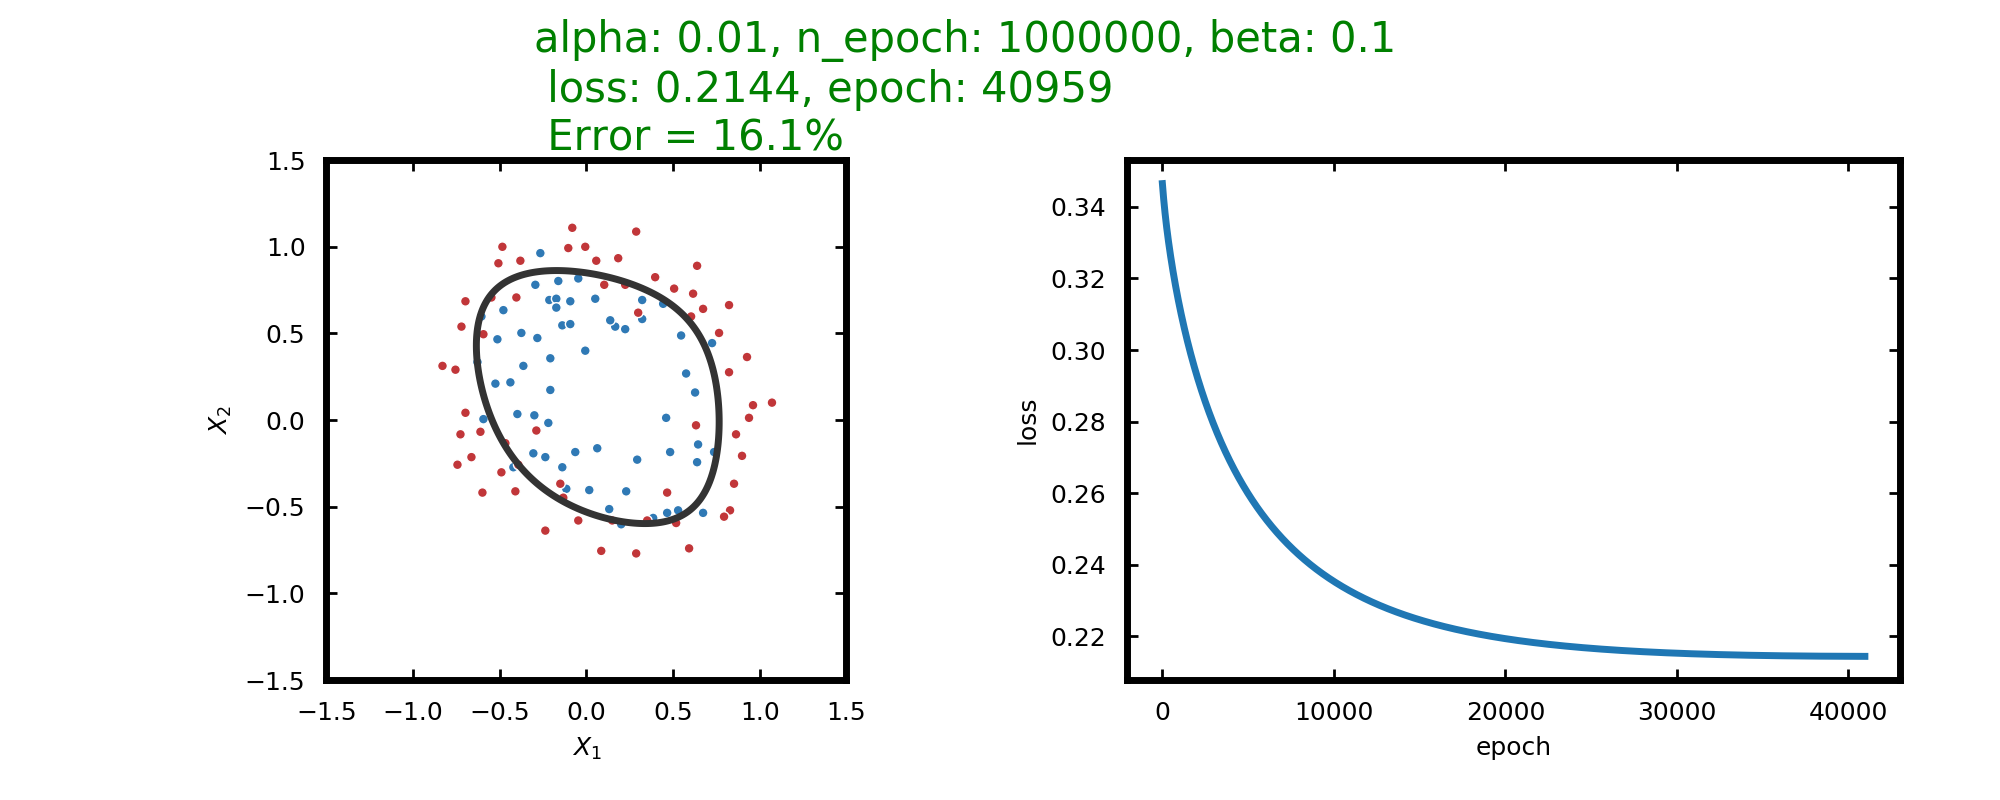
\includegraphics[width=0.85\textwidth]{fig/prob3/alpha_0_01_n_epoch1000000_beta_0_1.png}
\centering 
\caption{\protect $\beta = 0.1$}
\label{fig:15th}
\end{figure}

\begin{figure}[H]
\centering
  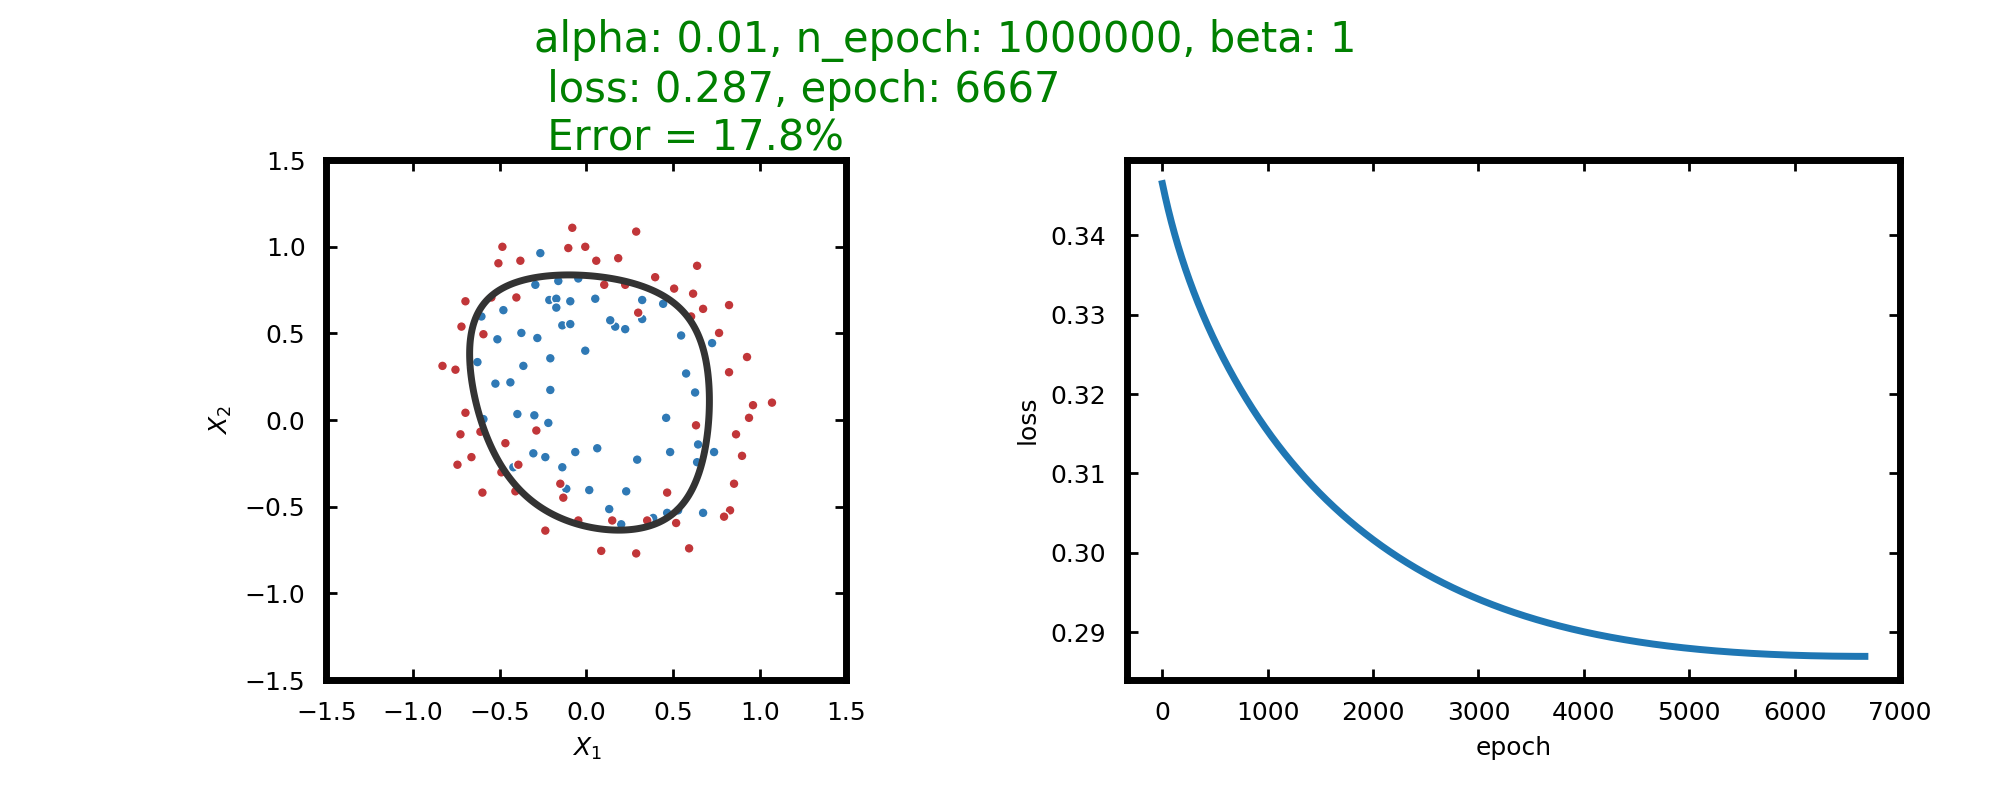
\includegraphics[width=0.85\textwidth]{fig/prob3/alpha_0_01_n_epoch1000000_beta_1.png}
\centering 
\caption{\protect $\beta = 1$}
\label{fig:15th}
\end{figure}

\begin{figure}[H]
\centering
  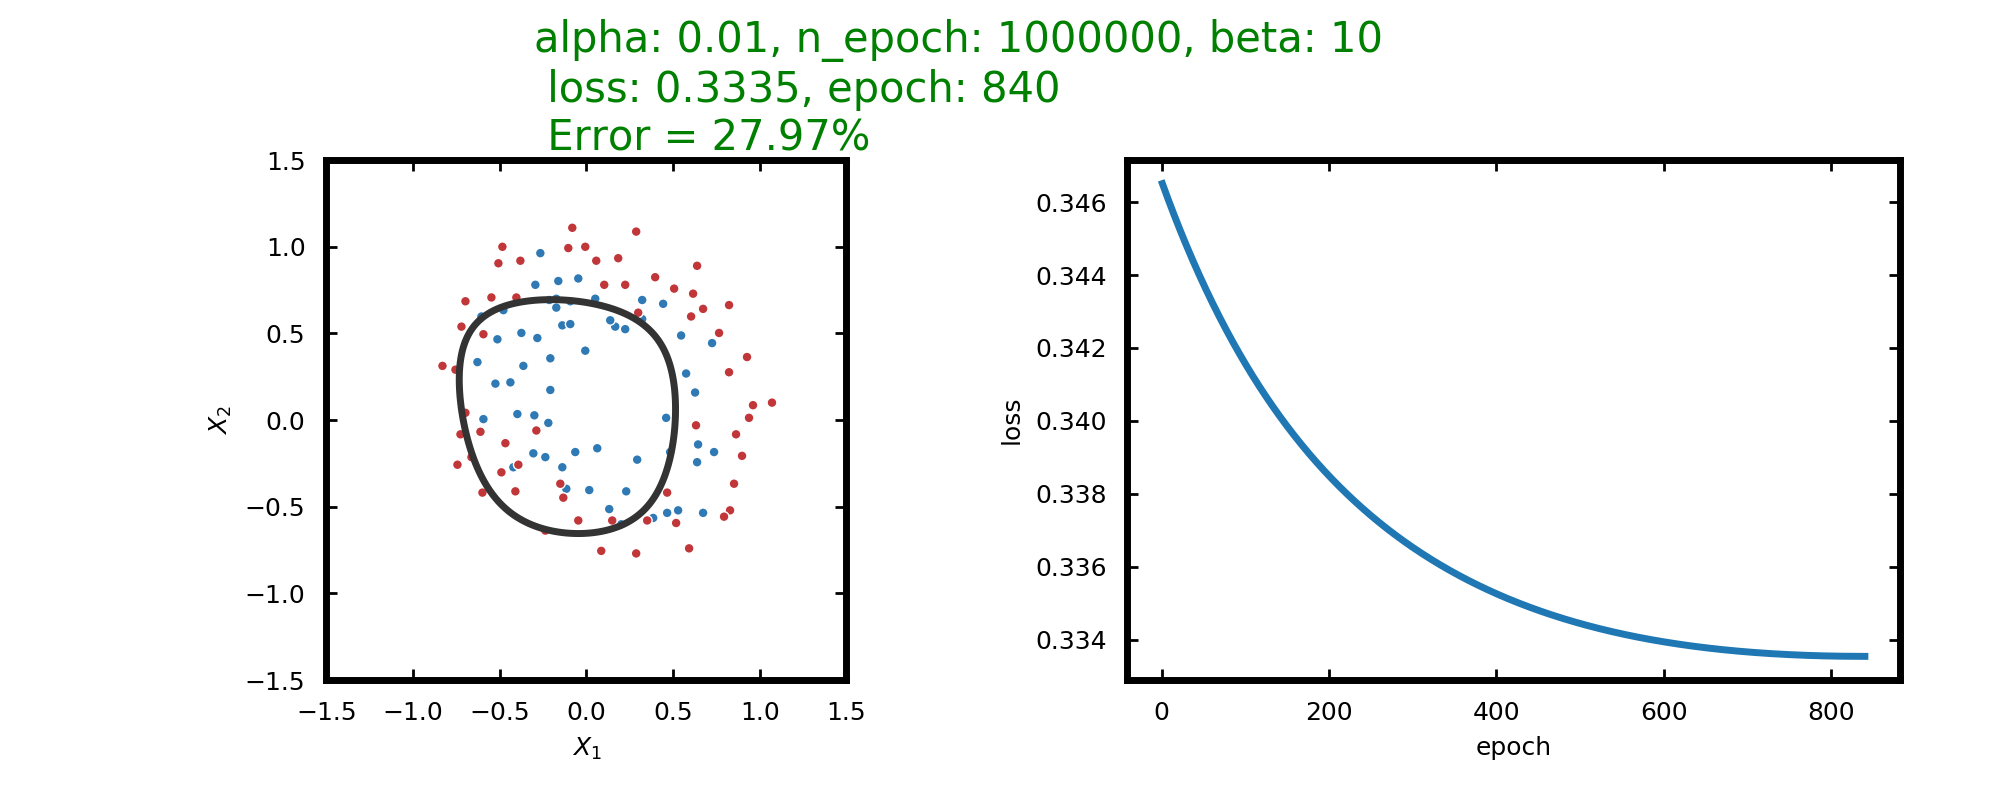
\includegraphics[width=0.85\textwidth]{fig/prob3/alpha_0_01_n_epoch1000000_beta_10.png}
\centering 
\caption{\protect $\beta = 10$}
\label{fig:15th}
\end{figure}

\begin{figure}[H]
\centering
  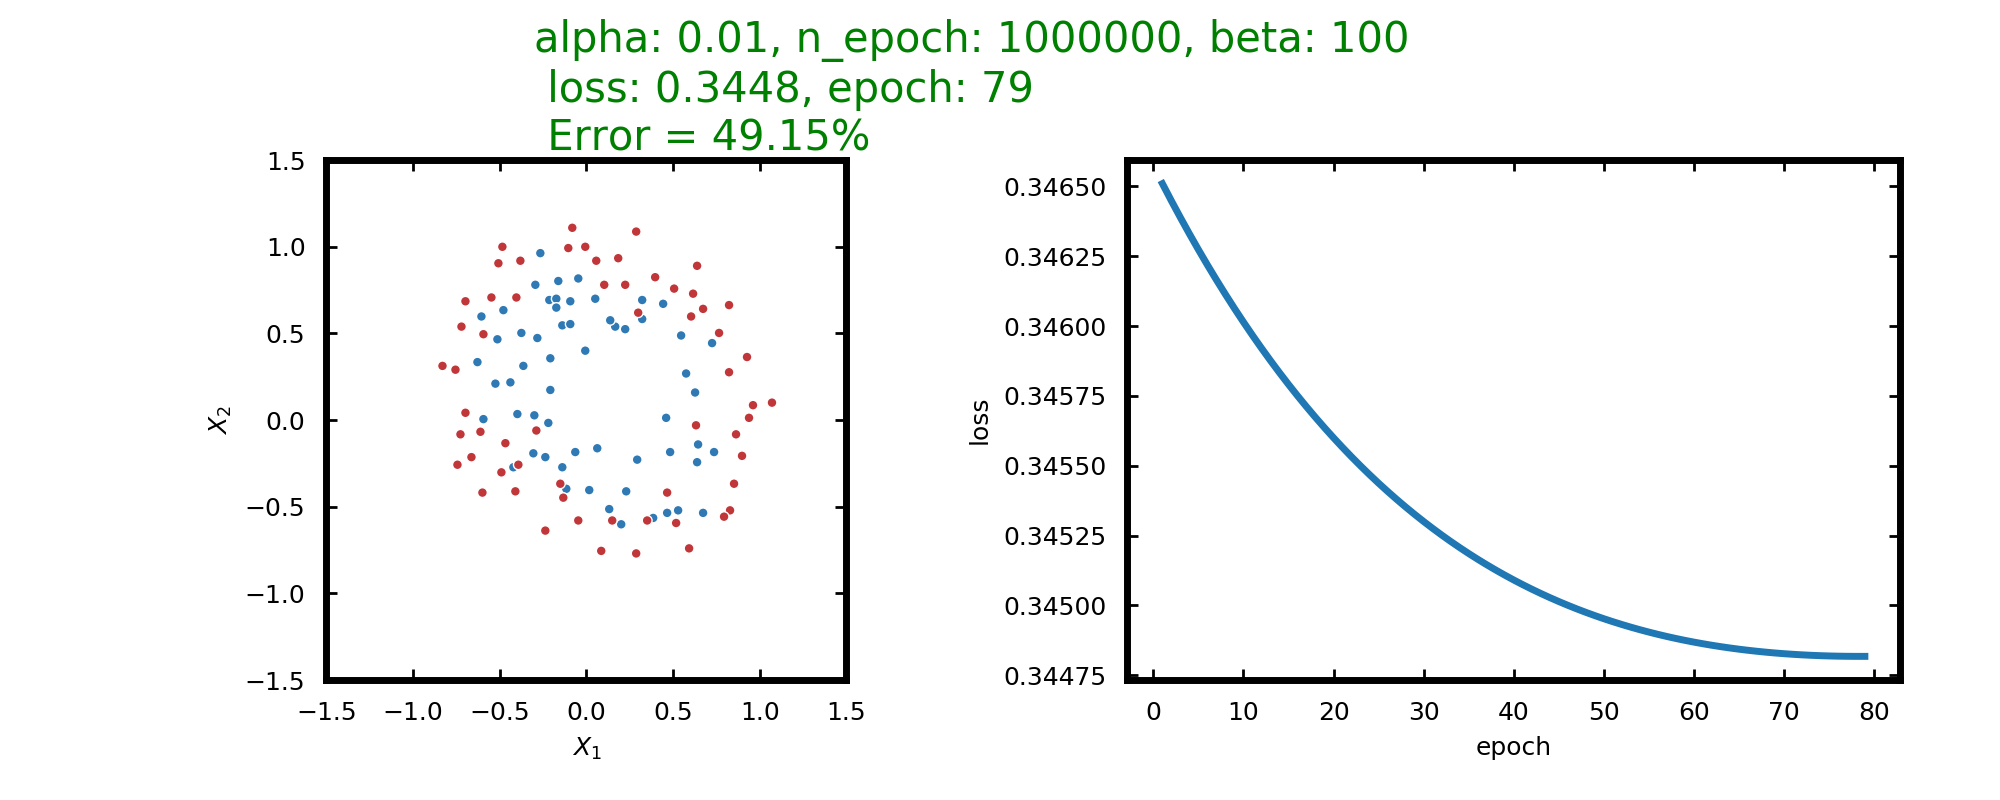
\includegraphics[width=0.85\textwidth]{fig/prob3/alpha_0_01_n_epoch1000000_beta_100.png}
\centering 
\caption{\protect $\beta = 100$}
\label{fig:15th}
\end{figure}





\end{document}
